\chapter{Introduction}
\label{ch:intro}

%===========================================================================================
%\section{History}
%===========================================================================================
%\subsection{Atomism}
%===========================================================================================
\section{The Standard Model}
According to the Standard Model (SM), all matter results from interactions between fundamental particles: lepton and quarks (fermions), and mediators (bosons).
Table \ref{tab:qrknlep} shows fermions of the standard model, their anti-particle equivalent would have all the signs reversed for the quantum numbers. For example, an anti-electron (\(e^+\)) and anti-electron-neutrino (\(\bar{\nu_e}\)) lepton number would flip to \((-1, 0, 0)\) and charges (\(Q\)s) would be \(+1\) and 0 respectively.

\begin{table}[htbp]
	\centering
	\begin{tabular}{c @{\hspace{5pt}} l |c|c|c|l|c|c|c|}
		% Top edges of both tables
		\cline{3-5} \cline{7-9}

		% Table Headers (overriding borders explicitly to ensure the outer walls exist)
		\multicolumn{2}{c|}{}              & \multicolumn{3}{c|}{Leptons} &              & \multicolumn{3}{c|}{Quarks}                                                                                         \\
		\cline{3-5} \cline{7-9}

		% Column Headers (merging the first two columns to center 'Category' with no borders)
		                                   &                              & \(l\)        & \(Q\)                       & \((L_e, L_\mu, L_\tau)\) &  & \(q\) & \(Q\)      & \((F_d, F_u, F_s, F_c, F_b, F_t)\) \\
		\cline{3-5} \cline{7-9}

		% Group A block
		\multirow{2}{*}{First generation}  & \ldelim\{{2}{*}              & \(e^-\)      & \(-1\)                      & (1, 0, 0)                &  & \(d\) & \(-1/3\)   & \((-1, 0, 0, 0, 0, 0)\)            \\
		                                   &                              & \(\nu_e\)    & 0                           & (1, 0, 0)                &  & \(u\) & \(2/3\)    & \((0, 1, 0, 0, 0, 0)\)             \\
		\cline{3-5} \cline{7-9}

		% Group B block
		\multirow{2}{*}{Second generation} & \ldelim\{{2}{*}              & \(\mu^-\)    & \(-1\)                      & (0, 1, 0)                &  & \(s\) & \( -1/3 \) & \((0, 0, -1, 0, 0, 0)\)            \\
		                                   &                              & \(\nu_\mu\)  & 0                           & (0, 1, 0)                &  & \(c\) & \(2/3\)    & \((0, 0, 0, 1, 0, 0)\)             \\
		\cline{3-5} \cline{7-9}

		% Group B block
		\multirow{2}{*}{Third generation}  & \ldelim\{{2}{*}              & \(\tau^-\)   & \(-1\)                      & (0, 0, 1)                &  & \(b\) & \(-1/3\)   & \((0, 0, 0, 0, -1, 0)\)            \\
		                                   &                              & \(\nu_\tau\) & 0                           & (0, 0, 1)                &  & \(t\) & \(2/3\)    & \((0, 0, 0, 0, 0, 1)\)             \\
		% Bottom edges of both tables                         
		\cline{3-5} \cline{7-9}
	\end{tabular}
	\label{tab:qrknlep}
	\caption{Three generations of leptons (left) and quarks (right).}
\end{table}
\begin{table}[htbp]
	\begin{tabular}{
		>{\centering\arraybackslash}m{2.8cm}
		>{\centering\arraybackslash}m{2.8cm}
		>{\centering\arraybackslash}m{2.8cm}
		>{\centering\arraybackslash}m{2.8cm}
		}

		% ROW 1: Strong Vertices
		\multicolumn{1}{c}{\vhead{Electromagnetic} }                                                      & \multicolumn{3}{l}{\vhead{Strong}} \\[0.1cm]
		\threevertex{fermion}{X^{+|-}}{fermion}{X^{-|+}}{photon}{\gamma}                                  &
		\threevertex{fermion}{q}{fermion}{q}{gluon}{g}                                                    &
		\threevertex{gluon}{g}{gluon}{g}{gluon}{g}                                                        &
		\fourvertex{gluon}{g}{gluon}{g}{gluon}{g}{gluon}{g}
		\\[1cm]

		% ROW 3: Electromagnetic and Electroweak Vertices
		\multicolumn{3}{l}{\vhead{Weak}}                                                                  &                                    \\[0.1cm]
		\threevertex{fermion}{\nu_e \mid \nu_\mu \mid \nu_\tau}{fermion}{e \mid \mu \mid \tau}{photon}{W} &
		\threevertex{fermion}{d/s/b}{fermion}{u/c/t}{photon}{W}                                           &
		\threevertex{fermion}{f}{fermion}{f}{photon}{Z}                                                   &



		\\[1cm]
		\multicolumn{2}{l}{\vhead{Electroweak}}                                                           & \multicolumn{2}{l}{\vhead{Higgs}}  \\[0.1cm]
		\threevertex{photon}{Z/\gamma}{photon}{W}{photon}{W}                                              &
		\fourvertex{photon}{W}{photon}{W}{photon}{W|Z/\gamma}{photon}{W|Z/\gamma}                         &
		\threevertex{fermion}{m}{fermion}{m}{scalar}{H}                                                   &
		\fourvertex{scalar}{H}{scalar}{H}{scalar}{m_B}{scalar}{m_B}
	\end{tabular}
	\caption{Feynman diagrams of various interaction vertices possible in the Standard Model}
	\label{tab:smvtx}
\end{table}

The mediators/bosons exchanged between the other fundamental particles give rise to the fundamental interactions: electromagnetism from the photon (\(\gamma\)), weak force from \(W^\pm\) and \(Z\) bosons, the gluon (\(g\)) for the strong force, and the Higgs boson (\(h\)) for imparting mass to the fundamental particles. Various interaction vertices possible in SM, that become the building blocks of all fundamental interactions are shown in \ref{tab:smvtx}. 

%===========================================================================================
\section{Quantum Chromodynamics}

%\subsection{Lagrangian and Feynman Rules}
\emph{Quantum Chromodynamics (QCD)} is the component of the SM which describes the strong interactions of quarks and gluons. The QCD Lagrangian can be expected as:
\begin{align}
	\mathcal{L}_\mathrm{QCD} = &\underbrace{\bar{q}^\alpha (i \gamma^\mu \partial_\mu\delta_{\alpha\beta} - g\gamma^\mu
	t^a_{\alpha\beta}A^a_\mu - m\delta_{\alpha\beta})q^\beta - \frac{1}{4} F^a_{\mu\nu}F_a^{\mu\nu}}_{\mathcal{L}_\mathrm{classical}}\notag\\ &\underbrace{- \frac{1}{2\lambda}(\partial^\mu A^a_\mu)^2}_{\mathcal{L}_\mathrm{gauge-fixing}}+ \underbrace{\bar{c}^\alpha\partial^\mu(\partial_\mu\delta_{\alpha\beta} + igT^a_{\alpha\beta}A^a_\mu)c^\beta}_{\mathcal{L}_\mathrm{ghost}}
\end{align}

\(\mathcal{L}_\mathrm{classical}\) is the classical Lagrangian density shows interaction of a quark field  \(q^\alpha\) with 3 color degrees of freedom interacting with gluon fields \(A^a_\mu\) with 8 color degrees of freedom. \(g\) and \(m\) are dimensionless and correspond to QCD coupling constant, and quark-mass respectively. \(F^a_{\mu\nu}\) are the gluon tensors defined as,
\begin{equation}
	F^a_{\mu\nu} = \partial_\mu A_\nu^a - \partial_\nu A_\mu^a - gf_{abc}A^b_\mu A^c_\nu.
	\label{eq:gluonFieldTensor}
\end{equation}

To properly define gluon propagators, we need to make a choice of gauge. The \(\mathcal{L}_\mathrm{gauge-fixing}\) parametrizes the class of covariant gauges with the gauge parameter $\lambda$. In non-Abelian theories, this gauge fixing term leads to creation of unphysical degrees of freedom, which are canceled out by \(\mathcal{L}_\mathrm{ghost}\) which contains complex, scalar fermion fields \(c^\alpha\). 

 The matrices \(t^a\) and  \(T^a\) are the fundamental and adjoint representations of \(\rm SU(3)\) in form of traceless \(3\times3\) and \(8\times8\) hermitian matrices satisfying:
\begin{align}
	[t^a, t^b] = if_{abc}t^c,~\tr(t^at^b) = \frac{1}{2}\delta^{ab} \notag\\
	[T^a, T^b] = if_{abc}T^c,~(T^{a})_{bc} = -if^{abc}.
\end{align}

Comparing with quantum electrodynamics (QED), where the photon field tensor lacks the last term of Eqn. \ref{eq:gluonFieldTensor} as it is an Abelian, \(U(1)\) gauge theory, we can explain the presence of three/four-gluon vertices and absence of such vertices for the photon in Table \ref{tab:smvtx}. The lagrangian can be used to formulate \emph{Feynman rules} for calculating amplitude contributions from various propagators and vertices, which are collected in Tab.~\ref{tab:qcdrules} of Appendix~\ref{app:qcdProcesses}. 

\subsection{The Running Coupling}
\label{subsec:runningCoupling}
At an energy scale \(Q\), consider a dimensionless observable \(X\). Lets assume that \(Q\) is sufficiently high that the quark masses become negligible in comparison. To calculate \(X\) as a perturbation series in the QCD coupling \(\alpha_s = \frac{g^2}{4\pi}\) (analogous to the QED fine structure constant), we need to remove ultraviolet divergences through renormalization. Renormalization introduces another arbitrary energy scale $\mu$ where the divergences are subtracted.  In general, \(X\) would depend on the ratio \(Q^2/\mu^2\) and post-renormalization coupling $\alpha_s(\mu^2)$. However, any physical observable should be independent of $\mu$:
\begin{align}
	\mu^2\frac{d X(Q^2/\mu^2, \alpha_s(\mu^2))}{d\mu^2} &= \left[\mu^2\frac{\partial}{\partial\mu^2} +  \mu^2\frac{\partial\alpha_s(\mu^2)}{\partial\mu^2}\frac{\partial}{\partial\alpha_s}\right] X(Q^2/\mu^2, \alpha_s(\mu^2)) = 0 \notag\\
	\implies & \left[-\frac{\partial}{\partial t} + \beta(\alpha_s) \frac{\partial}{\partial\alpha_s}\right] X(e^t, \alpha_s) = 0.
	\label{eqn:renormX}
\end{align} 

Where, \(t = \ln{\frac{Q^2}{\mu^2}}\), \(\beta(\alpha_s) = \mu^2\frac{\partial\alpha_s}{\partial\mu^2}\), \(\alpha_s\equiv\alpha_s(\mu^2(t))\)
\begin{align}
	\beta(\alpha_s) &= -\frac{\partial\alpha_s}{\partial t} \implies  t =  \int^{\alpha_s(Q^2)}_{\alpha_s}\frac{d\alpha_s}{\beta(\alpha_s)}\notag\\
			\implies & \frac{\partial\alpha_s(Q^2)}{\partial t} = Q^2\frac{\partial \alpha_s}{\partial Q^2}  =  \beta(\alpha_s(Q^2)), \quad\frac{\partial\alpha_s(Q^2)}{\partial\alpha_s} = \frac{\beta(\alpha_s(Q^2))}{\beta(\alpha_s)}
					\label{eq:runningCouplingIntro}
\end{align}

Substituting in Eq. \ref{eqn:renormX}, we see that \(X(1, \alpha_s(Q^2))\) is a valid solution. Thus the scale dependence in \(X\) comes from the \emph{running coupling} \(\alpha_s(Q^2)\).  Perturbatively expanding \(\beta(\alpha_s)\), we can write the \emph{renormalization group equation} as,

\begin{align}
Q^2\frac{\partial \alpha_s}{\partial Q^2}  = -\alpha_s^2(Q^2)\left(\beta_0 + \beta_1\alpha_s(Q^2) + \mathcal{O}(\alpha_s^2(Q^2))\right)
\label{eq:RGEquation}
\end{align}

Where,
\begin{equation}
	\beta_0 = \frac{1}{(4\pi)^2}\left(11 - \frac{2}{3}N_f\right), \quad \beta_1 =  \frac{1}{(4\pi)^4}\left(102 - \frac{38}{3}N_f\right)
\end{equation}

\begin{figure}[!htbp]
	\centering
	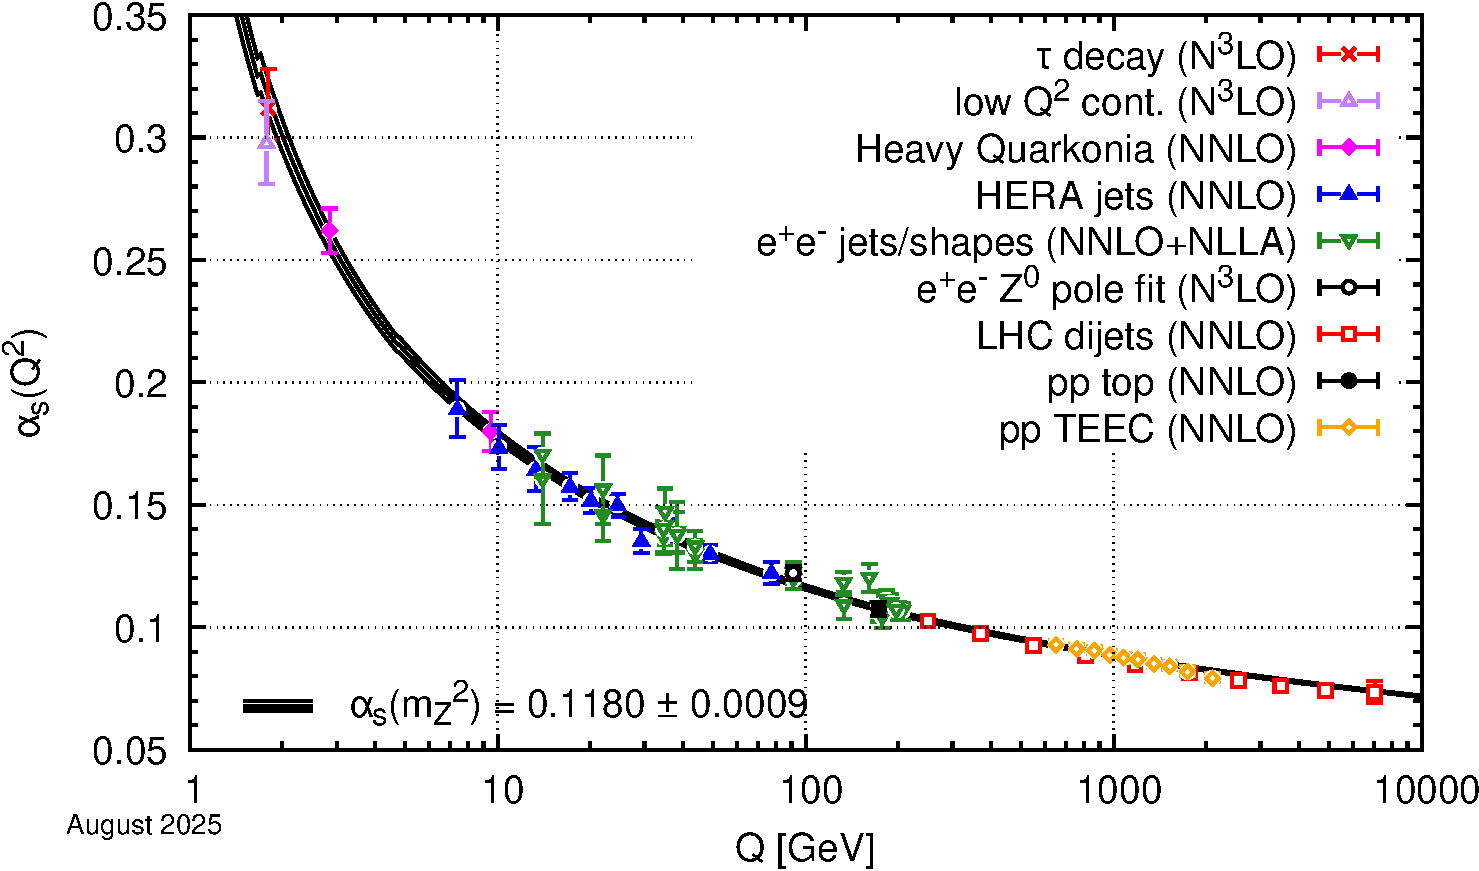
\includegraphics[width=0.7\linewidth]{figures/alphas-v-Q-2025-cropped.pdf}
	\caption{Summary of determinations of \(\alpha_s\) as a function of the energy scale Q compared to
		the running of the coupling computed at five loops taking as an input the current Particle Data Group (PDG) world average, \(\alpha_s(m_Z^2) = 0.1180 \pm 0.0009\) \cite{ParticleDataGroup:2026aaa}}
	\label{fig:runningCoupling}
\end{figure}

Integrating Eq. \ref{eq:RGEquation}
\begin{align}
	\ln(\frac{Q^2}{Q_0^2})  &= \int^{\alpha_s(Q^2)}_{\alpha_s(Q^2_0)}\frac{d\alpha_s}{\beta(\alpha_s)}\notag\\
	\implies \alpha_s(Q^2) &= \frac{\alpha_s(Q_0^2)}{1 + \beta_0(\alpha_s(Q_0^2))\ln(Q^2/Q_0^2) + \mathcal{O}(\alpha_s^2)}
	\label{eq:runningCouplingRel}
\end{align}

Usually, the reference scale \(Q_0^2\) is set to a convenient energy scale in the perturbative regime. \(\alpha_s\) at all other scales can be inferred accordingly. Usually, \(Q_0\) is set to mass of the \(Z\)-boson, \(m_Z\) as shown in Fig. \ref{fig:runningCoupling}. Another approach is to choose a scale parameter, \(\Lambda\) such that \(\alpha_s(\Lambda) \rightarrow \infty\).  

\begin{align}
	\ln(\frac{Q^2}{\Lambda^2}) &= - \int_{\alpha_s(Q^2)}^{\infty} \frac{d\alpha_s}{\beta(\alpha_s)}  \notag\\
	\implies \alpha_s(Q^2)  &= \frac{1}{\beta_0\ln(Q^2/\Lambda^2)}\left[1 - \frac{\beta_1}{\beta_0}\frac{\ln(\ln(Q^2/\Lambda^2))}{\ln(Q^2/\Lambda^2)} + \mathcal{O}\left(\frac{1}{\ln(Q^2/\Lambda^2)^2}\right)\right]
		\label{eq:runningCouplingLambda}
\end{align}

\(\Lambda\) is called the \emph{confinement scale}, around \(200~\mathrm{MeV}\). Eqs. \ref{eq:runningCouplingRel} and \ref{eq:runningCouplingLambda} show a monotonically decreasing relationship between \(\alpha_s\) and \(Q^2\). At high momentum transfers (\(Q \gg \Lambda\)), the coupling strength vanishes ($\alpha_s \to 0$). In this regime, quarks and gluons behave as quasi-free particles, making perturbative QCD (pQCD) calculations highly reliable (\emph{Asymptotic Freedom}).  At low energy scales (\(Q \ll \Lambda\)), the coupling diverges. In this non-perturbative QCD (npQCD) limit, isolated color charges cannot exist and partons are permanently bound into color-neutral hadrons (\emph{Color Confinement}).

\subsection{Quark Gluon Plasma (QGP)}
\label{sec:QGPIntro}
Asymptotic freedom of QCD means that matter at extremely high temperatures and densities (high \(Q^2\)) undergo a \emph{deconfinement} phase transition, with partonic degrees of freedom replacing hadronic degrees of freedom. 
%
This state of deconfined quarks and gluons is called QCD/quark-gluon plasma due to analogous phenomena observed in atomic physics~\cite{SHURYAK198071}.

Thermodynamically, when temperature (\(T\)) or baryon number density (\(n_\mathrm{B}\)) approaches the confinement scale \(\Lambda\) introduced in Sec.~\ref{subsec:runningCoupling} (\(T \sim \Lambda \sim \mathcal{O}(10^{12})K,~\text{and}~n_\mathrm{B} \sim \Lambda^3 \sim 1~\text{fm}^{-3}\)) the boundaries between hadrons become ill defined resulting in hadrons ``melt'' into QGP~\cite{Fukushima_2010}.  
%
For reference, the core of our sun ``only'' has \(T\sim \mathcal{O}(10^{7})K\) and \(n_\mathrm{B}\sim\mathcal{O}(10^{-14})\text{fm}^{-3}\). 

These orders of \(T\) and \(n_\mathrm{B}\) are the theorized conditions prevalent in the universe a few \(\mu\mathrm{s}\) after Big-Bang. The only natural phenomena in the present-day, cold universe that can achieve these conditions are the cores of neutron stars~\cite{Annala_2020} or neutron star mergers~\cite{neutronStarMerger}. Artificially, the required  \(T\) and \(n_\mathrm{B}\) can be achieved at facilities like the Large Hadron Collider (LHC) and Relativistic Heavy Ion Collider (RHIC) through collisions of heavy-ions (like Au, Pb, etc.) at near-light speeds, the aptly named \emph{little bangs}. More on this will be discussed in Sec. \ref{sec:heavyIonCollisions}. 

\section{Hard Processes}
To consider any nucleus as a singular coherent object, the fluctuations inside it would involve momentum transfers below the confinement scale (\(\Lambda\)) introduced in \ref{subsec:runningCoupling}, and would occur over timescales \(\sim 1/\Lambda\). We define \emph{hard-scattering processes} or just \emph{hard processes} as interactions of a hard perturbative probe with high momentum transfer \(Q >> \Lambda\). Since this interaction occurs over a time-scale \(\sim 1/Q \ll 1/\Lambda\), the perturbative probe effectively interacts with a near-static ``snapshot'' of the nucleus with a characteristic resolution \(\sim 1/Q\). 

\begin{figure}[htbp]
	\centering
	\factorizationdiagram
	\caption{Collinear factorization of a hadronic hard scattering.}
	\label{fig:factorization}
\end{figure}

Thus, the cross sections of a collision process of nuclei with momentum \(P_1\) and \(P_2\) depicted by Fig.~\ref{fig:factorization} can be \emph{factorized} into various independent components as,

\begin{equation}
	\frac{d\sigma}{d\mathbf{O}}  = \sum_{i,j,f} \int dx_1dx_2d\mathbf{\Phi}_ff_i(x_1, \mu^2)f_j(x_2, \mu^2)\frac{d\hat{\sigma}_{ij\to f}}{d\hat{\mathbf{O}}}D_f(\hat{\mathbf{O}}\to\mathbf{O}, \mu^2)
	\label{eq:factorization}
\end{equation}

Where, the interactions occur between partons \(i\) from nucleus 1 and \(j\) from nucleus 2 carrying momentum \(p_1 = x_1P_1\) and \(p_2 = x_2P_2\) respectively. \(\mu\) is an arbitrary \emph{factorization scale}, often just set to \(Q\). The \(f_{k}(x, \mu^2)\) are the \emph{parton densities} giving likelihood of a parton \(k\) to carry \(x\) fraction of it's parent nucleus's momentum at a particular factorization scale \(\mu\). \(f\) labels the partonic final state coming out of the scattering and \(\mathbf{\Phi}_f\) is its phase space. \(\hat{\sigma}_{ij\to f}\)  is the \emph{parton cross-section} for scattering of partons \(i\) and \(j\) into \(f\), kept differential in a partonic observable \(\hat{\mathbf{O}}\). We can approximate it to the \((n+k)\) order in \(\alpha_s\) as, 

\begin{equation}
	\frac{d\hat{\sigma}_{ij\to f}}{d\hat{\mathbf{O}}} = \alpha_s^k \sum_{m=0}^{n}\alpha_s^m\,\frac{d\hat{\sigma}^{(m)}_{ij\to f}}{d\hat{\mathbf{O}}}(p_1, p_2, Q^2/\mu^2)
	\label{eq:partonXsecOrders}
\end{equation}

Different hard processes will have different leading powers \(k\). \(W\) production will have \(k=0\) whereas perturbative dijet production with two outgoing quarks will have \(k=2\). 

The \(D_f(\hat{\mathbf{O}}\to\mathbf{O}, \mu^2)\) are the \emph{fragmentation functions}, giving the likelihood of a partonic final state with \(\hat{\mathbf{O}}\) being measured as \(\mathbf{O}\) once hadronization is over.
%
Like the parton densities, they cannot be calculated in perturbation theory, but they are \emph{universal}: once measured in one process they can be used in any other, and their dependence on \(\mu\) is governed by evolution equations of the same form as eq.~\ref{eq:RGEquation}.
%
Eq.~\ref{eq:factorization} is the skeleton of every measurement presented in this thesis, with the choice of \(\mathbf{O}\) being what separates one from the next, and a measurement is comparable to a calculation only if both use the same \(\mathbf{O}\).
%
Restricting \(\mathbf{O}\) to charged particles, as will be done for the angularities of Ch.~\ref{ch:angularities}, puts that restriction into \(D_f\) as well, and the non-perturbative input can then no longer be avoided.
%
The nuclear modification factors of Ch.~\ref{ch:hic} are ratios of Eq.~\ref{eq:factorization} between two collision systems, where the parton densities largely cancel and what is left is the effect of the medium on \(\hat{\sigma}_{ij\to f}\) and \(D_f\). 

%The parton densities \(f_i(x,\mu^2)\) in Eq.~\ref{eq:factorization} are not calculable in perturbation theory, but they are \emph{universal}: once measured in one process they may be used to predict any other. Requiring the physical cross section of Eq.~\ref{eq:factorization} to be independent of the arbitrary scale \(\mu\), exactly as for the coupling in Sec.~\ref{subsec:runningCoupling},
%\begin{equation}
%	\mu^2\frac{d}{d\mu^2}\,\sigma(P_1,P_2) = 0,
%	\label{eq:pdfRGE}
%\end{equation}
%ties the \(\mu\)-dependence of the densities to that of \(\hat{\sigma}_{ij}\).

\section{From partons to jets}
\label{sec:partonShower}
Outgoing partons evolve from higher to lower momentum transfer scales (say, \(t\)). Initially their evolution are modeled using the pQCD mechanism called \emph{parton shower}. Eventually, say at an infra-red scale cut-off \(t_0\), pQCD calculations stop being valid and npQCD processes like hadronization dominate. QCD Monte-Carlo programs combining parton shower at \(t < t_0\) and hadronization process at \(t > t_0\)  are called \emph{QCD event generators}


\subsection{Parton branching}
\label{subsec:dglap}
\begin{figure}[h]
\centering
\label{fig:splitKinematics}
\begin{tikzpicture}[>=latex, line width=0.6pt,]
	\node[draw,circle, minimum size=1cm, inner sep=2pt] (rest) at (-1,0) {\(\mathcal{M}_\mathrm{n}\)};
	\coordinate (splitPoint) at (0.5, 0);
	\coordinate (continual) at (2,0);
	\coordinate (splitUp) at (2, 1);
	\coordinate (splitDown) at (2, -1);
	\draw (rest) to [edge label=a] (splitPoint);
	\path[draw, dash pattern=on 2pt off 3pt on 4pt off 4pt] (splitPoint) -- (continual);
	\path[draw] (splitPoint) to [edge label=b] (splitUp);
	\path[draw] (splitPoint)  to [edge label'=c] (splitDown);
	
	\pic[draw, "\(\theta_a\)",  ->, angle eccentricity=1.7] {angle = continual--splitPoint--splitUp};
	\pic[draw, "\(\theta_b\)",  <-, angle eccentricity=2.] {angle = splitDown--splitPoint--continual};
\end{tikzpicture}
\hspace{1cm}
\begin{tikzpicture}[>=latex, line width=0.6pt]
	%\node[draw,circle, minimum size=1cm, inner sep=2pt, pattern=north west lines] (rest) at (-1,0) { };
	\coordinate (incoming) at (-1, 0);
	\coordinate (splitPoint) at (0.5, 0);
	\coordinate (continual) at (2,0);
		\node[draw,circle, minimum size=1cm, inner sep=2pt] (rest) at (2,1) {\(\mathcal{M}_\mathrm{n}\)};
	\coordinate (splitDown) at (2, -1);
	\draw (incoming) to [edge label=a] (splitPoint);
	\path[draw, dash pattern=on 2pt off 3pt on 4pt off 4pt] (splitPoint) -- (continual);
	\path[draw] (splitPoint) to [edge label=b] (rest);
	\path[draw] (splitPoint)  to [edge label'=c] (splitDown);
	
	\pic[draw, "\(\theta_a\)",  ->, angle eccentricity=1.7] {angle = continual--splitPoint--splitUp};
	\pic[draw, "\(\theta_b\)",  <-, angle eccentricity=2.] {angle = splitDown--splitPoint--continual};
\end{tikzpicture}
\caption{Kinematics of timelike (left) vs spacelike (right) parton branching}
\end{figure}

Consider nearly collinear timelike splitting of a parton, \(a\to b+c\) shown in Fig. \ref{fig:splitKinematics}. Let's assume the partons are massless, and define the evolution scale (\(t\)) as, 
\begin{align}
	t \equiv p_a^2 \approx 2E_bE_c(1 - \cos\theta)  \approx z(1-z)E_a^2\theta^2
\end{align}
Where, \(z = E_b/E_a = 1 - E_c/E_a\) and \(\theta = \theta_a + \theta_b\) is the small opening angle.  The cross-section of a \(n\)-parton state branching into \(n+1\)-parton state~\cite{Ellis_Stirling_Webber_1996}
%processes can be calculated by considering \(n\)-parton matrix element.
%\begin{equation}
%	\label{eq:nPartonXsec}
%	d\sigma_n = \mathcal{F}|\mathcal{M}_n|^2d\mathbf{\Phi}_n
%\end{equation}
%
%Where \(\mathcal{F}\) is the initial-state flux factor and \(\mathbf{\Phi}_n\) is phase space of the \(n\)-parton final state. In the branching process the \(n\)-parton pre-split phase space volume element:
%
%\begin{equation}
%	d\mathbf{\Phi}_{n} = \ldots \frac{d^3\mathbf{p}_a}{2(2\pi)^3E_a}
%\end{equation}
%
%will be replaced by the \(n+1\)-parton phase space and the \(n+1\)-parton matrix element can be calculated from the \(n\)-parton matrix element. 
%\begin{align}
%	d\mathbf{\Phi}_{n+1} &= \ldots \frac{d^3\mathbf{p}_b}{2(2\pi)^3E_b} \frac{d^3\mathbf{p}_c}{2(2\pi)^3E_c} 
%	= d\mathbf{\Phi}_{n} \frac{1}{4(2\pi)^3}dtdzd\phi \notag\\
%	|\mathcal{M}_{n+1}\big|^2 &\sim \frac{8\pi\alpha_s}{t}CF|\mathcal{M}_n|^2
%\end{align}
%
%Substituting in Eq. \ref{eq:nPartonXsec} and integrating away the \(d\phi\), we get,
%
\begin{align}
	\label{eq:xsecBranching}
	%d\sigma_{n+1} &= d\sigma_n \frac{dt}{t}dz\frac{\alpha_s}{2\pi}\int\frac{d\phi}{2\pi}CF \notag\\
	d\sigma_{n+1} &= d\sigma_n \frac{dt}{t}dz\frac{\alpha_s}{2\pi} \hat{P}_{ba}
\end{align}

The \(\hat{P}_{ba}(z)\) are the \emph{unregularized Altarsi-Parisi splitting functions}, giving the probability of the branching \(a \to b + c\) with \(b\) taking a fraction \(z\) of \(a\)'s energy.
%
Their leading order forms are shown in Tab.~\ref{tab:splitfns}.
%
\(\hat{P}_{qq}\) diverges as \(z\to1\), \(\hat{P}_{gq}\) as \(z\to0\), and \(\hat{P}_{gg}\) at both ends, each of these limits being the emission of a soft gluon.
%
Only \(\hat{P}_{qg}\), the splitting of a gluon into a \(q\bar{q}\) pair, stays finite over the whole range of \(z\).
%
%This soft pole is what grooming procedures like SoftDrop (Sec.~\ref{sec:jetAlgo}) are built to remove from a measured jet.

Same equation would hold for the space-like case. 
%
To obtain the evolution equations, we can frame the evolution in terms of the change in parton distribution function \(f(x,t)\) when the evolution scale \(t\) goes from \(t\) to \(t+\delta t\),
%
\begin{align}
	\delta f_i(x, t) &= \delta f_\mathrm{in} - \delta f_\mathrm{out} \notag\\
	&=\frac{\delta t}{t} \sum_j \int_{0}^{1} dz \frac{\alpha_s}{2\pi} \left[\frac{\hat{P}_{ij}(z)}{z}f_j(x/z, t) - \hat{P}_{ji}f_i(x,t)\right]
 \end{align}
 %
The second term of the RHS gives \emph{Sudakov form factor}, which gives the probability of a parton \(i\) evolving from scale \(t\) to a softer scale \(t_0\) without a resolvable emission,
%
\begin{align}
	\Delta_i(t) \equiv \exp(-\sum_j\int_{t_0}^{t} \frac{dt^\prime}{t^\prime}\int dz\frac{\alpha_s}{2\pi} \hat{P}_{ji}(z))
\end{align}

We get the familiar DGLAP-like evolution equations,

\begin{align}
	t\frac{\partial}{\partial t}\left(\frac{f_i}{\Delta_i}\right) = \frac{1}{\Delta_i}\sum_j \int \frac{dz}{z}\frac{\alpha_s}{2\pi}
\hat{P}_{ij}(z)f_j(x/z, t)\end{align}


To deal with singularities corresponding to soft gluons at \(z\to 1\), we introduce an explicit infrared cut-off \(z < 1-\epsilon(t)\) .  Requiring the transverse momentum in timelike branching \(a\to bc\) to be positive, 
\begin{align}
	p_T^2 &= z(1-z)p_a^2 - (1-z)p_b^2 - zp_c^2 > 0 \notag\\
	\implies& z(1-z) > t_0/t \implies t_0/t < z < 1 - t_0/t
%	\implies&  z, 1-z > \epsilon(t) = \frac{1 - \sqrt{1-4t/t_0}}{2}\simeq t_0/t \notag\\
\end{align} 
and also, \(t > 2t_0\). Thus the Sudakov factors become,
%
\begin{align}
	\Delta_i(t) \equiv \exp(-\sum_j\int_{2t_0}^{t}
	\frac{dt^\prime}{t^\prime}
	\int_{t_0/t^\prime}^{1-t_0/t^\prime} dz
	\frac{\alpha_s}{2\pi} \hat{P}_{ji}(z))
	\label{eq:col`inearSudakov}
\end{align}

\subsection{Angular Ordering}
\label{sec:angularOrdering}
Sec.~\ref{subsec:dglap} took collinear enhancements into account to all orders in
\(\alpha_s\). However it does not take the enhancement in soft gluon emission at wide emission angle. 
This is demonstrated in Eq. \ref{eq:softPropagator} by considering an on-mass-shell external line of
momentum \(p\), mass \(m\) emitting a gluon with momentum \(q\)  at an angle \(\theta\)
\begin{equation}
	\frac{1}{(p\pm q)^2 - m^2} = \frac{\pm1}{2p\cdot q}
	= \frac{\pm1}{2\omega E(1-v\cos\theta)},
	\label{eq:softPropagator}
\end{equation}
where \(\omega\) is the gluon energy, \(E\) and \(v\) the energy and velocity of the
emitter and \(\theta\) the emission angle. For light partons \(v\to1\) and the
collinear enhancement appears as \(\theta\to0\); the enhancement as \(\omega\to0\)
holds for any velocity and angle. Internal lines  are off-mass-shell and carry no such enhancement, since
\((p+q)^2-m^2\to p^2-m^2\neq0\). The cross section carries a sum over all pairs of external lines \(\{i,j\}\),
\begin{align}
	\label{eq:antennaSplitXSec}
	d\sigma_{n+1}& = d\sigma_n\,\frac{d\omega}{\omega}\frac{d\Omega}{2\pi}
	\frac{\alpha_s}{2\pi}\sum_{i,j}C_{ij}W_{ij}
\end{align}
The weighted sum \(\sum_{i,j}C_{ij}W_{ij}\)  is called the \emph{antenna pattern} of the process. The \emph{color factor} \(C_{ij}\) and \emph{radiation function} \(W_{ij}\)  are defined as,
\begin{align}
	C_{ij} &= -\mathbf{Q}_i\cdot\mathbf{Q}_j  \notag \\
	W_{ij} &= \frac{\omega^2 p_i\cdot p_j}{p_i\cdot q\;p_j\cdot q}
	= \frac{1-v_iv_j\cos\theta_{ij}}
	{(1-v_i\cos\theta_{iq})(1-v_j\cos\theta_{jq})}
\end{align}
  The vectors \(\mathbf{Q}_{i}\) represents color charge of parton \(i\). 
  %\(\mathbf{Q}_i^2 = C_F\) for a quark, \(C_A\) for a gluon and \(0\) for a color singlet. 
  \begin{equation}
  	\mathbf{Q}_i^2 = 
  	\begin{cases}
  		C_F = 4/3 & i \in \text{quarks} \\[-15pt]
  		C_A = 3 & i \in \text{gluons}\\[-15pt]
  		0 & i \in \text{color singlet}
  	\end{cases}
  \end{equation}
  
  \(W_{ij}\) comes from interference between lines \(i\) and \(j\). \(W_{ij}\) can be separated into two parts  \(W^{[i/j]}_{ij}\) each with an \emph{incoherent} and a \emph{coherent} contribution from line \(i/j\)  . Assuming massless emitters (\(v_i=v_j=1\)) for simplicity,
\begin{align}
	W_{ij} &= W^{[i]}_{ij} + W^{[j]}_{ij}\notag\\
	W^{[i]}_{ij} &= \frac{1}{2}\left(\overbrace{\frac{1}{1-\cos\theta_{iq}}}^\mathrm{incoherent} + \overbrace{\frac{\cos\theta_{iq}-\cos\theta_{ij}}{(1-\cos\theta_{jq}) (1-\cos\theta_{iq})}}^\mathrm{coherent}\right)\notag\\
	&=  \frac{1}{2(1-\cos\theta_{iq})}\left(1 + \frac{\cos\theta_{iq}-\cos\theta_{ij}}{1-\cos\theta_{ij}\cos\theta_{iq} - \sin\theta_{ij}\sin\theta_{iq}\cos\phi_{iq}}\right)
	\label{eq:antennaSplit}
\end{align}
Using the direction of line \(i\) as the z-axis, \(d\Omega \)  from Eq. \ref{eq:antennaSplitXSec} becomes \(d\cos\theta_{iq}\,d\phi_{iq}\), We can carry out the \(\phi_{iq}\) integration,
\begin{align}
	\int_0^{2\pi}\frac{d\phi_{iq}}{2\pi}W^{[i]}_{ij} &= \frac{1}{1-\cos\theta_{iq}}\left(\frac{1 + \frac{\cos\theta_{iq}-\cos\theta_{ij}}{|\cos\theta_{iq}-\cos\theta_{ij}|}}{2}\right) \notag\\
	&= \begin{cases}
		\dfrac{1}{1-\cos\theta_{iq}} & \cos\theta_{iq} > \cos\theta_{ij} \implies \theta_{iq} < \theta_{ij}\\[-10pt]
		0 & \text{otherwise,}
	\end{cases}
	\label{eq:angularOrdering}
\end{align}

Eq.~\ref{eq:angularOrdering}  shows that azimuth-averaged soft gluon emission from a line \(i\) is confined to a cone, centered on \(i\)'s direction, extending up to the direction of line \(j\), \(i\)'s sibling from the preceding split. 
%
Since the emission probability of Eq.~\ref{eq:antennaSplitXSec} is weighted by the color charges, a gluon radiates \(C_A/C_F = 9/4\) times as much as a quark of the same energy into the same cone.
%
Gluon jets are therefore wider and carry more particles than quark jets of the same momentum, a difference the classifiers of Ch.~\ref{ch:methods} are trained to pick up, and one that has to be kept in mind whenever angularities are compared between samples with different quark and gluon fractions.
%The total soft gluon emission cross-section can be then easily obtained for two external lines forming a color singlet (\(e^+e^-\to q\bar{q}\)) have \(\mathbf{Q}_i+\mathbf{Q}_j=0\) and hence \(C_{q\bar{q}}=\mathbf{Q}_q^2=\mathbf{Q}_{\bar{q}}^2 = C_F\), and angular ordering suppresses radiation outside the cones extending from \(q\) to \(\bar{q}\) and vice versa.

%\begin{align}
%	d\sigma_{q\bar{q}g}& = d\sigma_{q\bar{q}}\frac{\Theta(\cos(\theta_{qg})-\cos(\theta_{q\bar{q}}))}{1-\cos\theta_{qg}}d(\cos\theta_{qg})\frac{\alpha_s}{2\pi}\frac{d\omega}{\omega}C_F
%	\label{eq:qqbarSinglet}
%\end{align}
%We will come back to Eq.~\ref{eq:qqbarSinglet} 

\subsection{Color Coherence}
\label{sec:colorCoherence}
Lets take the case of three partons \(\{i,j,k\}\) forming a color singlet (\(\mathbf{Q}_i + \mathbf{Q}_j +\mathbf{Q}_k = 0\)) e.g., \(e^+e^-\to q\bar{q} g\). First, partons \(l\) and \(k\) come from a color singlet state (\(\mathbf{Q}_l +\mathbf{Q}_k = 0\)). Then \(l\) splits into \(i\) and \(j\) (\(\mathbf{Q}_l = \mathbf{Q}_i + \mathbf{Q}_j = -\mathbf{Q}_k\)). The antennae function for this state is:
\begin{align}
		\label{eq:threePartonW}
  \sum_{a,b}C_{ab}W_{ab} &= -\mathbf{Q}_i\!\cdot\!\mathbf{Q}_jW_{ij} -\mathbf{Q}_j\!\cdot\!\mathbf{Q}_kW_{jk} -\mathbf{Q}_i\!\cdot\!\mathbf{Q}_kW_{ik} \notag\\
	&= \frac{1}{2}\left[\mathbf{Q}_i^2(W_{ij} + W_{ik} - W_{jk}) + \mathbf{Q}_j^2(W_{ij} + W_{jk} - W_{ik}) + \mathbf{Q}_k^2(W_{ik} + W_{jk} - W_{ij})\right]\notag\\
	&=\mathbf{Q}_i^2\left(W_{ij}^{[i]} + \tilde{W}_{jk}^{[i]} - \tilde{W}_{ik}^{[j]}\right) + \mathbf{Q}_j^2\left(W_{ij}^{[j]} + \tilde{W}_{ik}^{[j]} - \tilde{W}_{jk}^{[i]}\right) \notag\\
	& + \mathbf{Q}_k^2\left(\tilde{W}_{jk}^{[i]} + \tilde{W}_{ik}^{[j]} + \frac{W_{ik}^{[k]} + W_{jk}^{[k]} }{2}\right)
\end{align}
Where,
\begin{equation}
	\tilde{W}_{jk}^{[i]} = \frac{W^{[i]}_{ik} - W^{[i]}_{ij}}{2},\quad \tilde{W}_{ik}^{[j]} = \frac{W^{[j]}_{jk} - W^{[j]}_{ij}}{2}
\end{equation}
are shifted radiation functions for lines \(i\) and \(j\), with the collinear singularity canceled out. This allows us to make certain useful approximations. Taking \(\theta_{ij}\to0\), we can approximate the directions of \(i\) and \(j\) by \(l\). 
\begin{align}
	W_{ik}^{[k]} \simeq W_{jk}^{[k]} \simeq W_{lk}^{[k]},\text{and}~\tilde{W}_{jk}^{[i]} \simeq \tilde{W}_{ik}^{[j]} \simeq W_{lk}^{[ij]}/2 
\end{align}
Where, 
\begin{equation}
	\tilde{W}^{[ij]}_{lk} = \begin{cases}
		W^{[l]}_{lk} & \theta_{lq}>\theta_{ij}\\[-10pt]
		0            & \theta_{lq}<\theta_{ij},
	\end{cases}
\end{equation}
\begin{equation}
	W \simeq \mathbf{Q}_i^2W^{[i]}_{ij} + \mathbf{Q}_j^2W^{[j]}_{ij}
	+ \mathbf{Q}_k^2W^{[k]}_{lk} + \mathbf{Q}_l^2\tilde{W}^{[ij]}_{lk},
	\label{eq:coherentPattern}
\end{equation}

\begin{figure}[htbp]
	\centering
	\begin{tikzpicture}[line width=0.55pt, scale=0.76,
		gl/.style={decorate, decoration={coil, aspect=0, segment length=1.7mm,
				amplitude=0.7mm}, ->}]
		
		\begin{scope}[xshift=0cm]
			\coordinate (o) at (0,0);
			\coordinate (l) at (35:1.05);
			\coordinate (i) at (46:2.2);
			\coordinate (j) at (21:2.2);
			\coordinate (k) at (-40:2.25);
			\draw[black] (l) -- (i) node[black, above=-2pt] {\(i\)};
			\draw[black] (l) -- (j) node[black, right=0pt] {\(j\)};
			\draw (o) -- node[above left=-5pt, pos=0.55] {\(l\)} (l);
			\draw (o) -- (k) node[below right=-4pt] {\(k\)};
			\coordinate (e) at ($(l)!0.55!(i)$);
			\fill (e) circle (1.1pt);
			\draw[gl] (e) -- ($(e)+(-35:1.75)$) node[below right=-4pt] {\(q\)};
			%\node at (1.1,-2.1) {\(\mathcal{M}_i\)};
		\end{scope}
		
		\node at (3.8,0.3) {\(+\)};
		
		\begin{scope}[xshift=4.6cm]
			\coordinate (o) at (0,0);
			\coordinate (l) at (35:1.05);
			\coordinate (i) at (46:2.2);
			\coordinate (j) at (21:2.2);
			\coordinate (k) at (-40:2.25);
			\draw[black] (l) -- (i) node[black, above=-2pt] {\(i\)};
			\draw[black] (l) -- (j) node[black, right=0pt] {\(j\)};
			\draw (o) -- node[above left=-5pt, pos=0.55] {\(l\)} (l);
			\draw (o) -- (k) node[below right=-4pt] {\(k\)};
			\coordinate (e) at ($(l)!0.55!(j)$);
			\fill (e) circle (1.1pt);
			\draw[gl] (e) -- ($(e)+(-35:1.75)$) node[below right=-4pt] {\(q\)};
			%\node at (1.1,-2.1) {\(\mathcal{M}_j\)};
		\end{scope}
		
		\node at (8.4,0.3) {\(\simeq\)};
		
		\begin{scope}[xshift=9.2cm]
			\coordinate (o) at (0,0);
			\coordinate (l) at (35:1.05);
			\coordinate (i) at (46:2.2);
			\coordinate (j) at (21:2.2);
			\coordinate (k) at (-40:2.25);
			\draw[black!30] (l) -- (i) node[black, above=-2pt] {\(i\)};
			\draw[black!30] (l) -- (j) node[black, right=0pt] {\(j\)};
			\draw (o) -- node[above left=-5pt, pos=0.55] {\(l\)} (l);
			\draw (o) -- (k) node[below right=-4pt] {\(k\)};
			\coordinate (e) at ($(o)!0.55!(l)$);
			\fill (e) circle (1.1pt);
			\draw[gl] (e) -- ($(e)+(-35:1.75)$) node[below right=-4pt] {\(q\)};
			%\node at (1.1,-2.1) {\(\mathcal{M}_l\)};
		\end{scope}
	\end{tikzpicture}
	\caption{Wide-angle emission of soft gluon \(q\), off \(i\) and \(j\), acts as if
	the emission came off the parent parton \(l\), imagined to be on shell.}
	\label{fig:threeParton}
\end{figure}


Each parton radiates in proportion to its color charge squared. When \(i\) and \(j\) close in angle their incoherent
contributions are limited to cones of half-angle \(\theta_{ij}\), while at larger
angles, out to the direction of \(k\), they radiate coherently in proportion to
their combined charge \(\mathbf{Q}_l^2\), as if from an internal line of momentum
\(p_l = p_i+p_j\) as shown in Fig.~\ref{fig:threeParton}.

\subsection{Coherent Parton Branching}
\label{sec:coherentPartonBranching}
Extended to higher orders this gives a \emph{coherent parton branching} formalism.
In place of the virtual mass-squared \(t\) the evolution variable is the opening
angle, or more precisely
\begin{equation}
	\zeta = \frac{p_b\cdot p_c}{E_bE_c} \simeq 1-\cos\theta
	\label{eq:zeta}
\end{equation}
for \(a\to bc\), with angular ordering \(\zeta^\prime<\zeta\) imposed on successive
branchings and the propagator factor \(dt/t\) of Sec.~\ref{subsec:dglap} replaced by
\(d\zeta/\zeta\). Using the splitting function \(\hat{P}_{ba}(z)dz\) rather than the
soft approximation \(\mathbf{Q}_a^2d\omega/\omega\) treats both soft and collinear
enhancements correctly, so that
\begin{equation}
	d\sigma_{n+1} = d\sigma_n\,\frac{d\zeta}{\zeta}\,dz\,
	\frac{\alpha_s}{2\pi}\hat{P}_{ba}(z).
	\label{eq:coherentBranching}
\end{equation}
The virtual mass-squared cut-off is replaced by an angular one,
\(\zeta_0 = t_0/E^2\) for a parton of energy \(E\), and the convenient evolution
variable \(\tilde{t} = E^2\zeta \geq t_0\) in terms of which the ordering condition \(\zeta_b,\zeta_c<\zeta_a\) and the
resulting cut-off on \(z\) read
\begin{equation}
	\tilde{t}_b < z^2\tilde{t},
	\qquad
	\tilde{t}_c < (1-z)^2\tilde{t},
	\qquad
	\sqrt{t_0/\tilde{t}} < z < 1-\sqrt{t_0/\tilde{t}} ,
	\label{eq:orderingCutoff}
\end{equation}
with \(\tilde{t}=\tilde{t}_a\) and \(z=E_b/E_a\). Neglecting the masses of \(b\) and
\(c\),
\begin{equation}
	t = z(1-z)\tilde{t},
	\qquad
	p_t^2 = z^2(1-z)^2\tilde{t},
	\label{eq:tAndPt}
\end{equation}
and the Sudakov form factor of Sec.~\ref{subsec:dglap} becomes
\begin{align}
	\tilde{\Delta}_i(\tilde{t}) \equiv \exp(-\sum_j\int_{4t_0}^{\tilde{t}}
	\frac{d\tilde{t}^\prime}{\tilde{t}^\prime}
	\int_{\sqrt{t_0/\tilde{t}^\prime}}^{1-\sqrt{t_0/\tilde{t}^\prime}} dz
	\frac{\alpha_s(z^2(1-z)^2\tilde{t}^\prime)}{2\pi} \hat{P}_{ji}(z))
	\label{eq:coherentSudakov}
\end{align}

At large \(\tilde{t}\) this falls more slowly than its collinear counterpart, though
still faster than any negative power of \(\tilde{t}\). The slower fall implies less
branching, which is the suppression of soft gluon emission by angular ordering.

\subsection{Angular structure of a jet}
\label{sec:angularityEstimate}
Sec.~\ref{sec:coherentPartonBranching} is enough to estimate what the radiation around a hard parton looks like. 
%
At a hadron collider, the angle \(\theta\) between two particles is measured as their distance \(\Delta R\) in the \etaphi plane and the energy \(E\) as the transverse momentum \(p_\mathrm{T}\) (see Sec.~\ref{sec:detCoordSys}), and a \emph{jet} is, for now, all the radiation within \(\Delta R < R\) of the initiating parton. 
%
Taking \(z\) to be the momentum fraction of the emitted gluon, as in \(\hat{P}_{gq}\) and \(\hat{P}_{gg}\) of Tab.~\ref{tab:splitfns}, the soft limit is \(\hat{P}_{gi}(z) \to 2C_i/z\) and \(d\zeta/\zeta \to 2d\theta/\theta\), so Eq.~\ref{eq:coherentBranching} becomes,
\begin{equation}
	dP = \frac{2\alpha_s C_i}{\pi}\frac{d\hat{\theta}}{\hat{\theta}}\frac{dz}{z}, \qquad \hat{\theta} \equiv \frac{\Delta R}{R} < 1
	\label{eq:lundDensity}
\end{equation}
Where, \(C_i = \mathbf{Q}_i^2\) is the color charge of the initiating parton from Sec.~\ref{sec:angularOrdering}. 
%
Eq.~\ref{eq:lundDensity} is flat in \(\ln(1/z)\) and \(\ln(1/\hat{\theta})\), so a jet is filled uniformly in this plane, the \emph{Lund plane}, down to the cut-off. 
%
The \emph{generalized angularity} of a jet is the sum over its emissions,
\begin{equation}
	\lambda_\beta = \sum_{i \in \mathrm{jet}} z_i\,\hat{\theta}_i^{\,\beta}
	\label{eq:angularityShower}
\end{equation}
Eq.~\ref{eq:LambdaKappaBeta} is the same quantity written in terms of the measured constituents of a jet, with \(z_i \to p_\mathrm{T, const}/p_\mathrm{T, jet}\) and \(\hat{\theta}_i \to \Delta R_\mathrm{const, jet}/R\), and with a second exponent \(\kappa\) on \(z_i\) which is \(1\) here. 
%
For \(\beta > 0\), an emission contributes nothing to \(\lambda_\beta\) in either the soft or the collinear limit, which is what makes it an IRC safe observable. 
%
Since \(\lambda_\beta\) is additive, the probability of a jet having an angularity below \(\hat{\lambda}_\beta\) is the probability of no emission with \(z\hat{\theta}^\beta > \hat{\lambda}_\beta\), which is the Sudakov form factor of Eq.~\ref{eq:coherentSudakov} with the no-emission condition replaced accordingly. 
%
Calling this cumulative distribution \(\Sigma_i(\hat{\lambda}_\beta)\), with the hat marking it as a parton level quantity like in Eq.~\ref{eq:factorization}, the hadron level cross section follows from it through the fragmentation function of Eq.~\ref{eq:factorization} for \(\mathbf{O} = \lambda_\beta\), summed over the flavor of the parton initiating the jet,
\begin{align}
	\frac{d\sigma}{d\lambda_\beta} &= \sum_{i \in \{q, g\}}\int d\hat{\lambda}_\beta\,\frac{d\sigma_i}{d\hat{\lambda}_\beta}\,D_i(\hat{\lambda}_\beta \to \lambda_\beta) = \sum_{i \in \{q, g\}}\sigma_i\int d\hat{\lambda}_\beta\,\frac{d\Sigma_i}{d\hat{\lambda}_\beta}\,D_i(\hat{\lambda}_\beta \to \lambda_\beta)
	\label{eq:angularityCumulant}
\end{align}
Where, \(\sigma_i\) is the cross section for producing a jet initiated by parton \(i\), i.e. Eq.~\ref{eq:factorization} with everything but the flavor of the outgoing parton integrated over, and \(d\sigma_i/d\hat{\lambda}_\beta = \sigma_i\,d\Sigma_i/d\hat{\lambda}_\beta\) is its parton level distribution. 
%
Normalized to the total cross section, the left hand side is the distribution measured in Ch.~\ref{ch:angularities}. 
%
The rest of this section is about \(\Sigma_i\), and comes back to \(D_i\) at the end. 
%
At fixed coupling,
\begin{align}
	\Sigma_i(\hat{\lambda}_\beta) &= \exp\left(-\frac{2\alpha_s C_i}{\pi}\int_0^1\frac{d\hat{\theta}}{\hat{\theta}}\int_0^1\frac{dz}{z}\,\Theta(z\hat{\theta}^\beta - \hat{\lambda}_\beta)\right) \notag\\
	&= \exp\left(-\frac{\alpha_s C_i}{\pi\beta}\ln^2\hat{\lambda}_\beta\right)
	\label{eq:angularitySudakov}
\end{align}
Quark and gluon jets differ only through \(C_i\), so \(\Sigma_g = \Sigma_q^{C_A/C_F}\)~\cite{Larkoski_2014}.
%
 A convenient choice for scale of \(\alpha_s\) is \(p_\mathrm{T, jet}R\), the largest transverse momentum an emission inside the jet can have. 
%

Tab.~\ref{tab:angularityEstimate} evaluates Eq.~\ref{eq:angularitySudakov} for the three \(\beta\) values measured in Ch.~\ref{ch:angularities}. 

\begin{table}[htbp]
	\centering
	\begin{tabular}{c c c c c}
		\toprule
		\multirow{2}{*}{\(\beta\)} & \multicolumn{2}{c}{median \(\hat{\lambda}_\beta\)} & \multicolumn{2}{c}{fraction with \(\hat{\lambda}_\beta > 0.1\)} \\
		\cmidrule(lr){2-3} \cmidrule(lr){4-5}
		 & quark & gluon & quark & gluon \\
		\midrule
		0.5 & 0.13  & 0.26  & 59\% & 87\% \\
		1   & 0.06  & 0.15  & 36\% & 64\% \\
		2   & 0.02  & 0.07  & 20\% & 40\% \\
		\bottomrule
	\end{tabular}
	\caption[Leading logarithmic estimates of jet angularities at RHIC]{Parton level median angularity and fraction of jets with \(\hat{\lambda}_\beta > 0.1\) from Eq.~\ref{eq:angularitySudakov} at \(\alpha_s = 0.2\), corresponding to \(p_\mathrm{T, jet} \approx 20~\mathrm{GeV}/c\) and \(R = 0.4\), for quark (\(C_F = 4/3\)) and gluon (\(C_A = 3\)) initiated jets.}
	\label{tab:angularityEstimate}
\end{table}

Median angularities are larger by  a factor of 2--3 for gluon jets compared to quark jets. 
%
Increasing \(\beta\) pushes both to smaller values and widens the gap between them, as the observable weighs the wide angle radiation more heavily. 
%
Going up in \(p_\mathrm{T, jet}\) only changes \(\alpha_s\) logarithmically, so the distributions are expected to narrow slowly. 

%Eq.~\ref{eq:lundDensity} only holds for emissions whose transverse momentum, \(k_\mathrm{T} \approx z\,p_\mathrm{T, jet}\Delta R\), is above the scale where \(\alpha_s\) stops being perturbative, and below it the emissions are replaced by hadronization, which is what \(D_i\) in Eq.~\ref{eq:angularityCumulant} accounts for. 
%%
%An emission with \(k_\mathrm{T}\) between \(\Lambda \approx 0.2\)~GeV and \(1\)~GeV sitting at the edge of the jet contributes \(k_\mathrm{T}/(p_\mathrm{T, jet}R) \approx 0.03\)--\(0.12\) to \(\lambda_\beta\) for any \(\beta\), which is as large as the medians of Tab.~\ref{tab:angularityEstimate}. 
%%
%Thus at RHIC energies the npQCD part of an angularity is not a small correction on top of the pQCD part, and it only falls as \(1/p_\mathrm{T, jet}\). 
%%
%This is why the angularity distributions measured in Ch.~\ref{ch:angularities} sit above these estimates by about this much, why removing the soft wide angle radiation by grooming (Sec.~\ref{sec:jetAlgo}) brings them closer, and why the event generators of Sec.~\ref{sec:eventGenerators} are tested there as much on their hadronization as on their showers. 
%
%These are leading logarithmic estimates at fixed coupling, and are indicative rather than predictions. 
%%
%Terms of order \(\alpha_s\ln(1/\lambda_\beta)\), coming from the running of \(\alpha_s\), hard collinear splittings, the recoil of the jet axis against the emissions for \(\beta \leq 1\), and radiation across the jet boundary, are all of order one half at these values. 
%%
%The angularities with \(\kappa \neq 1\) used for \AuAu collisions in Ch.~\ref{ch:angularities} are not IRC safe, and no estimate of this kind exists for them. 

\section{Hadronization and event generators}
\label{sec:eventGenerators}
Coherent branching does not only suppress soft emission, it also organizes the color flow of the shower.
%
Eq.~\ref{eq:coherentPattern} of shows that a pair of partons close in angle radiates as its parent, carrying the parent's charge, so the color of a branching is handed down the tree along with its momentum.
%
Applying this at every branching down to the cut-off \(t_0\), neighbouring partons are the ones that are color connected, and the final state has sorted itself into color singlet groups whose invariant masses are set by \(t_0\) and \(\Lambda\), and not by the scale of the hard process that started it.
%
This property is called \emph{preconfinement}~\cite{Ellis_Stirling_Webber_1996}.
%
The preconfined singlets can either decay directly into hadrons, giving the \emph{cluster} models~\cite{Webber:147786}, or stretch a confining color flux tube between color connected partons and break it up, giving the \emph{string} models~\cite{ANDERSSON198331}. 

QCD event generators chain these processes, matrix elements for the hard processes from eq.~\ref{eq:factorization}, parton showers, additional semi-hard scatterings among the remaining constituents of the incoming hadrons making up the \emph{underlying event}, hadronization, and finally the decays of unstable hadrons.
%
Everything below the hard process carries parameters that are not fixed by theory, and a set of values for them obtained by fitting to data is called a \emph{tune}.
%
Two generators starting from the same matrix element can therefore still disagree, and the spread between them is the usual way of gauging how much of a prediction is genuinely perturbative. 

This thesis uses PYTHIA~\cite{Sj_strand_2006} and HERWIG~\cite{Bellm:2015jjp}, which differ in how they deal with the coherence of Sec.~\ref{sec:coherentPartonBranching}.
%
HERWIG orders its shower in angle and imposes Eq.~\ref{eq:angularOrdering} directly, then hadronizes the preconfined singlets as clusters.
%
PYTHIA instead orders in transverse momentum and radiates off color dipoles rather than off individual partons, which suppresses soft wide-angle emission without ordering in angle at all, and hadronizes with strings.
%

Both generators are used with tunes made for RHIC energies~\cite{Skands_2010, PhysRevD.105.016011, adkins2019studying}, as the tunes in widest use are fitted mostly to LHC data and overshoot the underlying event at \sPP{200}{GeV}.
%
PYTHIA-6 and PYTHIA-8 share the string hadronization and the transverse-momentum ordered shower, and differ mainly in their treatment of multiple parton interactions, color reconnection and beam remnants, all of which control the multiplicity and the soft, wide-angle part of an event.
%

Ch.~\ref{ch:jhcorr} also uses JEWEL~\cite{Zapp:2013vla}, which adds scattering of the shower partons off a thermal medium to this picture.
%
The response of the detector to the generated particles is simulated separately using GEANT~\cite{Brun:1987ma}, and Ch.~\ref{ch:methods} describes how its effects are taken back out of a measurement.


\section{Outline of this thesis}
Angular ordering makes the angular distribution of energy inside a jet a record of the shower that produced it, with the wide-angle radiation coming from the early, hard splittings and the core of the jet being filled in later.
%
This thesis measures that distribution.
%
It is measured first in \pp collisions, where it is a test of the vacuum shower and a baseline, and then in \AuAu collisions, where a deviation from that baseline is the imprint of the medium the shower has gone through. 

Ch.~\ref{ch:STAR} describes RHIC and the STAR detector, in particular the TPC and the BEMC which measure the charged and neutral parts of a jet.
%
Ch.~\ref{ch:hic} defines jets as the output of a jet finding algorithm rather than as partons, introduces SoftDrop grooming, and sets up the quantities used to describe a heavy-ion collision: the Glauber picture of the initial state, centrality, the event plane, and the nuclear modification factors used to quantify jet quenching.
%
Ch.~\ref{ch:methods} collects the analysis techniques, mainly the classifiers used to tag jets and the unfolding procedure used to remove detector effects from a measured distribution.
%
Ch.~\ref{ch:jhcorr} presents jet-hadron correlations relative to the event plane in \AuAu collisions, which probe the dependence of energy loss on the path length traversed in the medium.
%
Ch.~\ref{ch:angularities} presents generalized angularities, inclusive and groomed, in \pp collisions and then in \AuAu collisions.
%
Ch.~\ref{ch:summary} summarizes both measurements and what they suggest about where to go next. 

%% =====================================================================
%  qgmutualinfo.tex -- A. J. Larkoski, J. Thaler, W. J. Waalewijn,
%  "Gaining (Mutual) Information about Quark/Gluon Discrimination",
%  JHEP 11 (2014) 129 [arXiv:1408.3122], recast in the notation of
%  chapters/intro.tex and chapters/angularities.tex.
%
%  WHERE IT GOES: as a section either at the end of Sec. 1.4
%  (sec:partonShower), after jetportrait.tex, or as the opening
%  theory section of Ch. \ref{ch:angularities}.  It is written as a
%  \section with \subsections, matching jetportrait.tex.
%
%  NOTATION MAP -- paper -> thesis:
%    \lambda^\kappa_\beta   -> same symbol, Eq. \ref{eq:LambdaKappaBeta}
%    e_\beta = \lambda^1_\beta -> written \lambda^1_\beta throughout
%    C_i (C_F, C_A)         -> \mathbf{Q}_i^2, intro.tex Sec. 1.4.2
%    \theta_i = R_i/R_0     -> \Delta R_{const,jet}/R
%    \Sigma_i(e)            -> \Sigma_i(\lambda), same
%    their \beta_0, \beta_1 -> the thesis' \beta_0 (eq:RGEquation)
%    P_{i\to ig}(z)         -> \hat{P}_{gi}(z), Table \ref{tab:splitfns}
%
%  LABELS ASSUMED TO EXIST (all currently live):
%    ch:intro, ch:angularities, sec:partonShower, subsec:dglap,
%    sec:coherentPartonBranching, tab:splitfns, eq:antennaSplitXSec,
%    eq:angularOrdering, eq:coherentSudakov, eq:runningCouplingLambda,
%    eq:RGEquation, eq:LambdaKappaBeta, fig:GroomingAndRg
%
%  IF jetportrait.tex IS UNCOMMENTED in intro.tex, three derivations
%  below become one-line callbacks instead:
%    eq:qgmiLLsudakov  == jetportrait's eq:angularitySudakov
%    the (u,v) plane   == jetportrait's Eq. (angularityDef), 2nd line
%    9/4 and delta_g   == jetportrait's eq:casimirRatio, eq:swWidth
%  I have kept them self-contained here, with a pointer, so the file
%  compiles against intro.tex as it stands today.  Labels are all
%  prefixed eq:qgmi.../fig:qgmi... so nothing collides with
%  jetportrait.tex or qgjets.tex.
%
%  BIBTEX: \cite{Larkoski_2014} already resolves -- but thesis.bib
%  contains THREE identical Larkoski_2014 entries (lines 101, 268,
%  3092).  BibTeX takes the first and warns on the rest; worth
%  deduplicating at some point.  Not touched here.
% =====================================================================

\section{Quark--gluon discrimination as an information problem}
\label{sec:qgmi}

Chapter~\ref{ch:intro} ended with a cascade whose every emission rate is
proportional to the squared colour charge \(\mathbf{Q}_i^2\) of whatever is
radiating. That single fact is the whole of quark--gluon discrimination at lowest
order, and it is also its ceiling. The purpose of this section is to make that
statement quantitative, following Larkoski, Thaler and
Waalewijn~\cite{Larkoski_2014}, who ask two questions that the cascade alone does
not answer: \emph{how much} separation does \(\mathbf{Q}_g^2/\mathbf{Q}_q^2=9/4\)
actually buy, and \emph{what has to be true} of an observable for it to do better.
The answers are, respectively, about a tenth of one bit, and that the observable
must resolve something in the jet other than its overall colour charge.

\subsection{The observable family, in the variables of Chapter~\ref{ch:intro}}
\label{subsec:qgmiFamily}

The paper's discriminants are exactly the generalized angularities of
Eq.~\ref{eq:LambdaKappaBeta},
\begin{equation}
	\lambda^\kappa_\beta = \sum_{c\,\in J} z_c^\kappa\,\theta_c^\beta ,
	\qquad
	z_c = \frac{p_{\mathrm{T},c}}{\sum_{c^\prime\in J}p_{\mathrm{T},c^\prime}} ,
	\qquad
	\theta_c = \frac{\Delta R_{c}}{R} ,
	\label{eq:qgmiAngularity}
\end{equation}
with \(0\le z_c,\theta_c\le1\) and both exponents non-negative. A single
two-parameter family contains most of the observables the quark--gluon literature
uses, at the four corners of Fig.~\ref{fig:qgmiLambdaSpace}: \(\lambda^0_0\) is
constituent multiplicity, \(\lambda^2_0\) is \(p_T^D\), \(\lambda^1_1\) is the jet
width (girth, broadening), and \(\lambda^1_2\) is thrust, i.e.\ jet mass squared
over energy squared. Raising \(\beta\) weights wide-angle radiation, raising
\(\kappa\) weights hard constituents; \(\beta\) reaches into the cascade's angular
ordering and \(\kappa\) into its energy sharing, and these are the two independent
handles Sec.~\ref{sec:coherentPartonBranching} provides.

\begin{figure}[htbp]
	\centering
	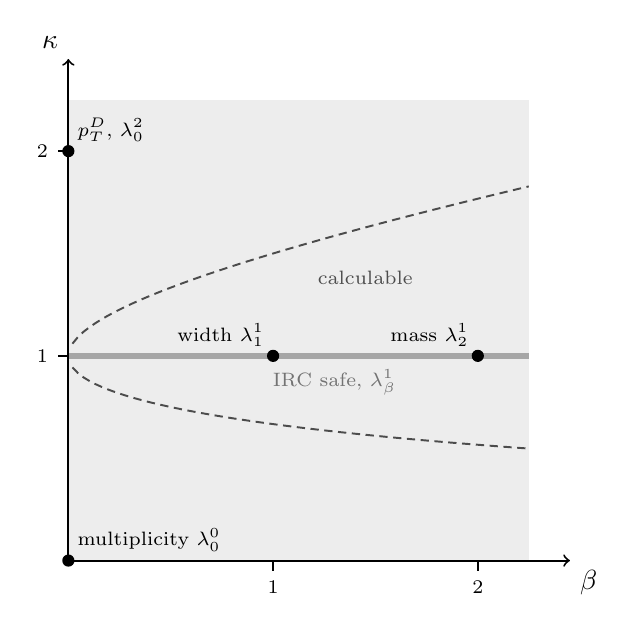
\begin{tikzpicture}[x=2.6cm, y=2.6cm, line width=0.7pt]
		\fill[black!7] (0,0) rectangle (2.25,2.25);
		% IRC-safe line kappa = 1
		\draw[line width=2.2pt, black!35] (0,1) -- (2.25,1);
		\node[black!55, font=\scriptsize] at (1.30,0.87)
		{IRC safe, \(\lambda^1_\beta\)};
		\draw[->] (0,0) -- (2.45,0) node[below right] {\(\beta\)};
		\draw[->] (0,0) -- (0,2.45) node[above left] {\(\kappa\)};
		\foreach \i in {1,2} {
			\draw (\i,0) -- (\i,-0.05) node[below] {\scriptsize\(\i\)};
			\draw (0,\i) -- (-0.05,\i) node[left] {\scriptsize\(\i\)};
		}
		\foreach \p/\l/\a in {%
			{0,0}/{multiplicity \(\lambda^0_0\)}/{above right},
			{0,2}/{\(p_T^D\), \(\lambda^2_0\)}/{above right},
			{1,1}/{width \(\lambda^1_1\)}/{above left},
			{2,1}/{mass \(\lambda^1_2\)}/{above left}} {
			\fill (\p) circle (2.2pt);
			\node[\a, font=\scriptsize, inner sep=3pt] at (\p) {\l};
		}
		% edge of the calculable region: 6(1-kappa)^2 = beta*kappa, i.e.
		% kappa = [(12+beta) +- sqrt((12+beta)^2-144)]/12
		\draw[densely dashed, black!70] plot[domain=0.02:2.25, samples=80]
		(\x, {((12+\x) - sqrt((12+\x)*(12+\x)-144))/12});
		\draw[densely dashed, black!70] plot[domain=0.02:2.25, samples=80]
		(\x, {((12+\x) + sqrt((12+\x)*(12+\x)-144))/12});
		\node[font=\scriptsize, black!70] at (1.45,1.38) {calculable};
	\end{tikzpicture}
	\caption[The space of generalized angularities]{%
		The \((\beta,\kappa)\) plane of Eq.~\ref{eq:qgmiAngularity}. The line
		\(\kappa=1\) holds the IRC safe angularities; the four marked points are the
		observables in common use. Inside the dashed contour,
		\(\beta\kappa/(1-\kappa)^2>6\) of Eq.~\ref{eq:qgmiBarrier}, the distribution
		is calculable from the cascade with a single non-perturbative number; outside
		it, an entire non-perturbative function is needed. Redrawn from
		Ref.~\cite{Larkoski_2014}.}
	\label{fig:qgmiLambdaSpace}
\end{figure}

Two features of Eq.~\ref{eq:qgmiAngularity} carry consequences that are easy to
miss and that both bear on Chapter~\ref{ch:angularities}.

\paragraph{Infrared and collinear safety sits at \(\kappa=1\) only.} Splitting a
constituent of momentum fraction \(z\) into two collinear pieces \(z_1+z_2=z\)
changes \(\sum z_c^\kappa\) by \(z_1^\kappa+z_2^\kappa-z^\kappa\), which vanishes
only for \(\kappa=1\). The \(\beta>0\) suppression handles the collinear region at
the \emph{jet axis} but not collinear splittings of a wide-angle constituent, so
\(\kappa\neq1\) is collinear unsafe everywhere in \(\beta\). This is the same
statement as the one made after Eq.~\ref{eq:LambdaKappaBeta}: restricting the sum
to charged tracks is a \(\kappa\)-like reweighting and costs IRC safety.
Sec.~\ref{subsec:qgmiUnsafe} is the machinery that buys it back.

\paragraph{The axis must be recoil-free.} Ref.~\cite{Larkoski_2014} measures
\(\Delta R_c\) to the \emph{winner-take-all} axis, not to the jet momentum axis.
The distinction is invisible at \(\beta\ge1\) but not below: with a momentum axis, a
single hard wide-angle emission displaces the axis itself, so \(\lambda^\kappa_\beta\)
measures the recoil of the initiating parton rather than the radiation pattern about
it, and the resummation acquires a second, spurious source of logarithms. Every
analytic statement below assumes a recoil-free axis. The measurement in
Chapter~\ref{ch:angularities} uses the standard jet axis, so the calculations quoted
here are a guide to the physics rather than a prediction to be overlaid on the data
--- unless the axis is changed.

The one kinematic picture used throughout is the cascade's own. Eq.~\ref{eq:antennaSplitXSec}
in the soft-collinear limit gives a single emitter the emission density
\begin{equation}
	dn = \frac{2\alpha_s\mathbf{Q}_i^2}{\pi}\frac{dz}{z}\frac{d\theta}{\theta}
	= \frac{2\alpha_s\mathbf{Q}_i^2}{\pi}\,du\,dv ,
	\qquad
	u = \ln\frac{1}{z} ,
	\qquad
	v = \ln\frac{1}{\theta} ,
	\label{eq:qgmiLundPlane}
\end{equation}
uniform on the quadrant \(u,v>0\) with a density set entirely by \(\mathbf{Q}_i^2\).
An emission contributes \(z^\kappa\theta^\beta = e^{-(\kappa u+\beta v)}\) to
Eq.~\ref{eq:qgmiAngularity}, so \(\lambda^\kappa_\beta>\lambda\) requires an emission
below the straight line \(\kappa u+\beta v=\ln(1/\lambda)\). Every result in this
section is a statement about that line and about the uniform density it cuts.

\subsection{Truth overlap: the right way to score a discriminant}
\label{subsec:qgmiMI}

The paper's organising quantity is the \emph{mutual information} between two
variables,
\begin{equation}
	I(A;B) = \int da\,db\;p(a,b)\log_2\frac{p(a,b)}{p(a)p(b)}
	= H(A)+H(B)-H(A,B) ,
	\label{eq:qgmiMIdef}
\end{equation}
with \(H\) the Shannon entropy, \(H(A)=-\sum_a p(a)\log_2p(a)\). Written the second
way it is manifestly the overlap area of two sets in Fig.~\ref{fig:qgmiVenn}:
\(H(A)\) and \(H(B)\) are the number of bits each variable carries, \(H(A,B)\) the
number the two carry together, and \(I(A;B)\) the bits they share. It vanishes iff
\(a\) and \(b\) are independent.

Now let \(T\) be the jet's flavour, \(t=0\) for a quark and \(t=1\) for a gluon, and
take a sample that is half of each, so that \(H(T)=1\): there is exactly one bit of
truth to be recovered, no matter how many bits an observable carries in total. The
\emph{truth overlap} of an observable is its mutual information with that bit,
\begin{equation}
	I(T;A) = \int d\lambda\left[
	\frac{p_q(\lambda)}{2}\log_2\frac{p_q(\lambda)}{p_{\rm tot}(\lambda)}
	+ \frac{p_g(\lambda)}{2}\log_2\frac{p_g(\lambda)}{p_{\rm tot}(\lambda)}\right] ,
	\qquad
	p_{\rm tot} = \frac{p_q+p_g}{2} ,
	\label{eq:qgmiTruthOverlap}
\end{equation}
bounded by \(0\le I(T;A)\le H(T)=1\), zero for two identical distributions and one
for two that do not overlap. It plays the role a ROC curve plays in an experimental
paper --- and indeed if one observable's ROC curve is everywhere better than
another's, its truth overlap is strictly larger, so nothing is lost by the change of
language --- but unlike a ROC curve it is a single number with a closed-form
integral, which is what makes the analytic study below possible.

\begin{figure}[htbp]
	\centering
	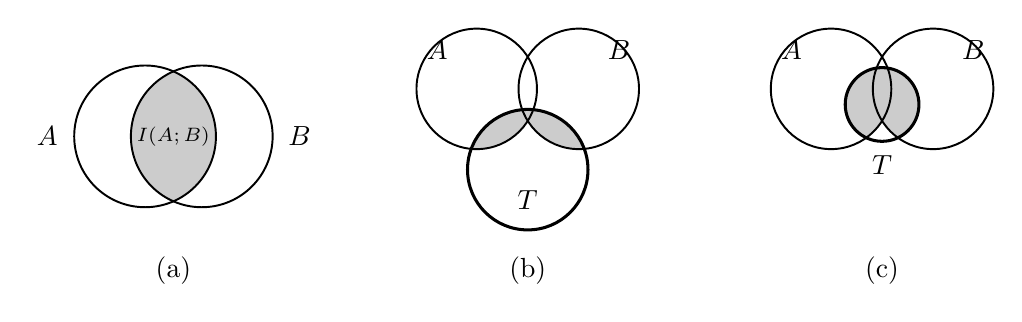
\begin{tikzpicture}[line width=0.7pt, scale=0.90,
		lens/.style={fill=black!20}]
		% ---- (a) I(A;B) ----
		\begin{scope}[yshift=-0.15cm]
			\begin{scope}
				\clip (-0.40,0) circle (1.00);
				\fill[lens] (0.40,0) circle (1.00);
			\end{scope}
			\draw (-0.40,0) circle (1.00);
			\draw (0.40,0) circle (1.00);
			\node at (-1.78,0) {\(A\)};
			\node at (1.78,0) {\(B\)};
			\node[font=\scriptsize] at (0,0) {\(I(A;B)\)};
			\node at (0,-1.90) {(a)};
		\end{scope}
		% ---- (b) complementary: A and B reach T in two different places ----
		\begin{scope}[xshift=5.0cm]
			\begin{scope}
				\clip (0,-0.62) circle (0.85);
				\fill[lens] (-0.72,0.52) circle (0.85);
				\fill[lens] (0.72,0.52) circle (0.85);
			\end{scope}
			\draw (-0.72,0.52) circle (0.85) node[above left=0.24cm] {\(A\)};
			\draw (0.72,0.52) circle (0.85) node[above right=0.24cm] {\(B\)};
			\draw[line width=1.1pt] (0,-0.62) circle (0.85);
			\node at (0,-1.05) {\(T\)};
			\node at (0,-2.05) {(b)};
		\end{scope}
		% ---- (c) redundant: same A and B, T moved onto their overlap ----
		\begin{scope}[xshift=10.0cm]
			\begin{scope}
				\clip (0,0.30) circle (0.52);
				\fill[lens] (-0.72,0.52) circle (0.85);
				\fill[lens] (0.72,0.52) circle (0.85);
			\end{scope}
			\draw (-0.72,0.52) circle (0.85) node[above left=0.24cm] {\(A\)};
			\draw (0.72,0.52) circle (0.85) node[above right=0.24cm] {\(B\)};
			\draw[line width=1.1pt] (0,0.30) circle (0.52);
			\node at (0,-0.55) {\(T\)};
			\node at (0,-2.05) {(c)};
		\end{scope}
	\end{tikzpicture}
	\caption[Mutual information and truth overlap]{%
		(a) Mutual information \(I(A;B)\), Eq.~\ref{eq:qgmiMIdef}, as the shared area
		of two variables in information space. (b) and (c): the observables \(A\) and
		\(B\) are drawn identically in the two panels, so their correlation
		\(I(A;B)\) is the same; only the truth bit \(T\) has moved. Shaded is the
		joint truth overlap \(I(T;A,B)\), the part of \(T\) reached by either
		observable. In (b) the two reach \(T\) in different places and the shaded
		region is much larger than the part either reaches alone, so combining them
		gains; in (c) they reach it in the same place, the shaded region is barely
		larger than either lobe, and combining them gains nothing. Correlation
		between observables and complementarity for discrimination are therefore
		separate questions. After Ref.~\cite{Larkoski_2014}.}
	\label{fig:qgmiVenn}
\end{figure}

The distinction the paper is built around is between \(I(A;B)\) and
\begin{equation}
	I(T;A,B) = H(T) + H(A,B) - H(T,A,B)
	\;\geq\; \max\left\{I(T;A),\,I(T;B)\right\} ,
	\label{eq:qgmiJoint}
\end{equation}
the truth overlap of the \emph{pair}. The first measures whether two observables are
correlated; the second measures whether their correlation, or lack of it, is of any
use. Figure~\ref{fig:qgmiVenn}(b) and (c) are drawn with identical \(I(A;B)\) and
identical individual truth overlaps and different \(I(T;A,B)\). This resolves a
standing puzzle in the substructure literature, where two variables are repeatedly
found to be weakly correlated and yet to gain nothing when combined: they are
uncorrelated in the bits that carry no flavour information and redundant in the bits
that do. The useful figure of merit is therefore the \emph{gain}
\begin{equation}
	\Delta I(T;A\to A,B) \equiv I(T;A,B) - \max\left\{I(T;A),I(T;B)\right\} ,
	\label{eq:qgmiGain}
\end{equation}
not the correlation coefficient.

\subsection{Casimir scaling, and why it caps the answer near a tenth of a bit}
\label{subsec:qgmiCasimir}

Call an observable \emph{Casimir scaling} if its cumulative distributions --- the
fraction of jets with the observable below \(\lambda\) --- take the form
\begin{equation}
	\Sigma_q(\lambda) = e^{-C_F\,r(\lambda)} ,
	\qquad
	\Sigma_g(\lambda) = e^{-C_A\,r(\lambda)}
	= \left[\Sigma_q(\lambda)\right]^{C_A/C_F} ,
	\label{eq:qgmiCasimir}
\end{equation}
for \emph{any} monotonic \(r\). The quark and gluon curves differ by a power, and by
nothing else: the observable has seen the jet's colour charge and no other property
of it. Equation~\ref{eq:qgmiCasimir} is the generic outcome of the cascade, because
Eq.~\ref{eq:qgmiLundPlane} puts \(\mathbf{Q}_i^2\) in front of the whole emission
density and nowhere else.

Cutting at \(\lambda<\lambda_{\rm cut}\) keeps a fraction \(x=\Sigma_q\) of quarks and
\(x^{C_A/C_F}\) of gluons, so the entire ROC curve is fixed,
\begin{equation}
	\varepsilon_g = \varepsilon_q^{\,C_A/C_F} = \varepsilon_q^{\,9/4} ,
	\label{eq:qgmiROC}
\end{equation}
independent of \(r\). The truth overlap is fixed with it, and the cleanest way to see
this is to note that Eq.~\ref{eq:qgmiMIdef} is invariant under any invertible change
of variable, so one may as well use \(\Sigma_q\) itself as the observable. Setting
\(\varrho\equiv C_A/C_F\) and \(w\equiv\Sigma_q(\lambda)\in[0,1]\), the quark
distribution of \(w\) is uniform by construction and the gluon distribution follows
from \(\Sigma_g=w^{\varrho}\),
\begin{equation}
	p_q(w) = 1 ,
	\qquad
	p_g(w) = \frac{d}{dw}w^\varrho = \varrho\,w^{\varrho-1} ,
	\label{eq:qgmiUniform}
\end{equation}
and every trace of the observable has disappeared. Substituting in
Eq.~\ref{eq:qgmiTruthOverlap},
\begin{equation}
	I(T;A) = \frac{1}{2}\int_0^1 dw\left[
	\log_2\frac{2}{1+\varrho w^{\varrho-1}}
	+ \varrho w^{\varrho-1}\log_2\frac{2\varrho w^{\varrho-1}}{1+\varrho w^{\varrho-1}}
	\right]
	\;\xrightarrow[\;\varrho=9/4\;]{}\;
	0.103 .
	\label{eq:qgmiBaseline}
\end{equation}
Every Casimir-scaling observable, whatever it measures and however well it is
measured, returns the same \(0.103\) of the one available bit. This is the number
against which everything else in this section is compared, and it is the quantitative
form of the remark closing Sec.~\ref{sec:coherentPartonBranching}: the separation is
statistical, the distributions overlap heavily, and the overlap is not an artifact of
any particular choice of observable.

The IRC safe angularities are Casimir scaling at leading logarithmic accuracy. An
emission carries \(\lambda^1_\beta\) above \(\lambda\) when \(u+\beta v<\ln(1/\lambda)\),
a triangle of area \(\ln^2(1/\lambda)/2\beta\) in the plane of
Eq.~\ref{eq:qgmiLundPlane}; vetoing every such emission, exactly as the Sudakov form
factor Eq.~\ref{eq:coherentSudakov} vetoes resolvable branchings, gives
\begin{equation}
	\Sigma_i(\lambda^1_\beta) = \exp\left[-\frac{\alpha_s}{\pi}
	\frac{\mathbf{Q}_i^2}{\beta}\ln^2\lambda^1_\beta\right] ,
	\label{eq:qgmiLLsudakov}
\end{equation}
which is Eq.~\ref{eq:qgmiCasimir} with \(r=(\alpha_s/\pi\beta)\ln^2\lambda\). So at
this order width, thrust and every angularity between them have \emph{identical}
discrimination power, \(0.103\) bits, and \(\beta\) has dropped out entirely. The
same is true, as Sec.~\ref{subsec:qgmiUnsafe} shows, of most of the IRC unsafe plane.
Casimir scaling is not a property of a few observables; it is what one gets by
default, and it explains the long-standing observation that wildly different
quark--gluon taggers perform almost identically.

\emph{Improving on \(0.103\) therefore requires resolving something in the jet other
than \(\mathbf{Q}_i^2\).}

\subsection{What breaks Casimir scaling}
\label{subsec:qgmiNLL}

Everything that distinguishes quark from gluon jets beyond the overall charge is
subleading in the logarithmic counting. Writing the cumulative distribution as
\begin{equation}
	\ln\Sigma(\lambda) = \underbrace{\alpha_s\ln^2\lambda}_{\rm LL}
	+ \underbrace{\alpha_s\ln\lambda}_{\rm NLL}
	+ \alpha_s + \mathcal{O}(\alpha_s^2) ,
	\label{eq:qgmiLogCounting}
\end{equation}
LL keeps the first term with \(\alpha_s\ln^2\lambda\sim1\), NLL adds the second.
Ref.~\cite{Larkoski_2014} evaluates Eq.~\ref{eq:qgmiTruthOverlap} on NLL
distributions of the form
\begin{equation}
	\Sigma_i(\lambda^1_\beta) =
	\frac{e^{-\gamma_E R_i^\prime}}{\Gamma(1+R_i^\prime)}\,
	e^{-R_i(\lambda^1_\beta)-\gamma_i T(\lambda^1_\beta)} ,
	\qquad
	R_i^\prime \equiv -\frac{dR_i}{d\ln\lambda^1_\beta} ,
	\label{eq:qgmiNLLcum}
\end{equation}
in which three distinct things spoil Eq.~\ref{eq:qgmiCasimir}, in increasing order of
physical interest.

\begin{enumerate}
	\item \textbf{The running coupling.} \(\alpha_s\) in Eq.~\ref{eq:qgmiLLsudakov} is
	really evaluated at the transverse momentum of each emission,
	\(\alpha_s(p_Tz\theta)\) --- Eq.~\ref{eq:runningCouplingLambda} with the scale
	fixed by Eq.~\ref{eq:tAndPt} --- so the radiator becomes a function of
	\(\lambda_\beta\equiv2\alpha_s\beta_0\ln\lambda^1_\beta\) rather than of
	\(\ln^2\lambda\). The exponent is still \(\propto\mathbf{Q}_i^2\), so this alone
	preserves Casimir scaling, but it sets the scale at which the other two act.

	\item \textbf{Multiple emissions.} The prefactor
	\(e^{-\gamma_ER^\prime}/\Gamma(1+R^\prime)\) corrects the LL assumption that a
	single emission dominates \(\lambda^1_\beta\); since
	\(R^\prime\propto\mathbf{Q}_i^2\) and \(\Gamma\) is not an exponential, this is a
	genuine, though mild, violation.

	\item \textbf{The hard-collinear splitting functions.} This is the physical one.
	\(\gamma_i\) in Eq.~\ref{eq:qgmiNLLcum} is the non-cusp anomalous dimension, which
	is nothing but the \(z\)-integral of the regularized splitting functions of
	Table~\ref{tab:splitfns} away from their soft poles,
	\begin{equation}
		\gamma_q = \frac{3}{4}C_F = 1 ,
		\qquad
		\gamma_g = \frac{11}{12}C_A - \frac{n_f}{6} = \frac{23}{12} ,
		\qquad
		\frac{\gamma_g}{\gamma_q} = \frac{23}{12} \neq \frac{9}{4} .
		\label{eq:qgmiNonCusp}
	\end{equation}
	A quark emits by \(\hat{P}_{qq}\) only; a gluon emits by \(\hat{P}_{gg}\) and
	splits by \(\hat{P}_{qg}\), and its \(n_f\) flavours of quark pair are a channel a
	quark jet does not have. In the soft limit \(z\to0\) all of these collapse to
	\(2\mathbf{Q}_i^2/z\) and only the charge survives, which is why LL sees only
	\(9/4\). At finite \(z\) they differ in \emph{shape}, and
	\(23/12\neq9/4\) is the first place the cascade remembers what opened the jet.
\end{enumerate}

The outcome is that \(I(T;\lambda^1_\beta)\) is no longer flat in \(\beta\): it rises
monotonically as \(\beta\) falls towards zero, reaching roughly \(0.11\)--\(0.13\) at
\(\beta\simeq0.5\) against the \(0.103\) LL baseline. Small \(\beta\) weights all
angles alike and so counts emissions rather than measuring their spread, moving the
observable towards multiplicity --- the best single discriminant in both parton
showers. In the plane of Eq.~\ref{eq:qgmiLundPlane} this is the statement that the
flavour information lives at large \(u\) and small \(v\), soft and wide-angle, which
is precisely the corner grooming removes; see Sec.~\ref{subsec:qgmiThesis}.

Two cautions come with this. The NLL result is a perturbative one and omits
non-perturbative power corrections, so it should not be trusted below
\(\beta\simeq0.5\). And when the same truth overlaps are extracted from
\textsc{Pythia}~8 and \textsc{Herwig}\texttt{++} the two disagree with each other and with NLL by amounts
comparable to the entire effect --- \textsc{Pythia}~8 systematically more optimistic, \textsc{Herwig}\texttt{++}
close to the LL baseline. The disagreement does \emph{not} appear when quark and
gluon distributions are compared individually; it appears only in their separation.
That is a warning about every Monte-Carlo-based estimate of tagging performance, and
the reason the paper's closing recommendation to the LHC experiments is for unfolded
angularity distributions over a range of \(\beta\) in purified samples.

\subsection{Charged-particle angularities: the weighted-energy function}
\label{subsec:qgmiUnsafe}

The measurement in Chapter~\ref{ch:angularities} restricts Eq.~\ref{eq:qgmiAngularity}
to tracks, which as noted there costs IRC safety. Ref.~\cite{Larkoski_2014} handles
the whole \(\kappa\neq1\) plane with the same device that makes track-based
observables calculable: factor the non-perturbative step into an object with a
perturbative evolution, exactly as Sec.~\ref{sec:partonShower} factors hadronization
out of the cascade.

The object is the \emph{weighted-energy function} \(F^i_\kappa(x,\mu)\), the
probability that a parton of flavour \(i\) fragments into a set of hadrons with
\(\sum_h z_h^\kappa = x\), normalized to \(\int_0^\infty dx\,F^i_\kappa(x,\mu)=1\).
It is the \(\kappa\)-weighted sibling of the fragmentation function \(D^h_i(x,t)\):
where \(D\) tracks one hadron's share of the parton's energy, \(F\) tracks the whole
final state's contribution to \(\lambda^\kappa_0\) in one number. For \(\kappa=1\)
restricted to charged particles it is the track function, and weighted by charge it
is the jet charge distribution. Being non-perturbative it must be measured, but it
evolves perturbatively with the splitting functions already in
Table~\ref{tab:splitfns},
\begin{equation}
	\mu\frac{\partial}{\partial\mu}F^i_\kappa(x,\mu)
	= \frac{1}{2}\sum_{j,k}\int dz\,dx_1\,dx_2\,
	\frac{\alpha_s}{\pi}\hat{P}_{i\to jk}(z)\,
	F^j_\kappa(x_1,\mu)F^k_\kappa(x_2,\mu)\,
	\delta\!\left(x - (1-z)^\kappa x_1 - z^\kappa x_2\right) ,
	\label{eq:qgmiFRGE}
\end{equation}
with the jet's own scale \(\mu=p_{\rm T}R\). Equation~\ref{eq:qgmiFRGE} is
Sec.~\ref{subsec:dglap}'s DGLAP equation with the convolution moved from the momentum
fraction into the observable: both daughters are kept, each carrying its own \(F\),
and the \(\delta\) function adds their contributions with the \(\kappa\)-weights the
observable demands. It is, in other words, the parton shower, written for this
observable. Measure \(F^i_\kappa\) once and Eq.~\ref{eq:qgmiFRGE} transports it to any
other jet \(p_{\rm T}\) or radius; the paper checks this against both showers for
\(p_T^D\).

The remarkable result is what happens for \(\beta>0\). Repeating the veto argument of
Eq.~\ref{eq:qgmiLLsudakov} with the emission now fragmenting, the radiator is
\begin{equation}
	R_i(\lambda^\kappa_\beta) = \int_0^1\frac{d\theta}{\theta}\int_0^1 dz\,
	\frac{\alpha_s(p_{\rm T}z\theta)}{\pi}\hat{P}_{gi}(z)
	\int_0^\infty dx\,F^g_\kappa(x,\mu)\,
	\Theta\!\left(x z^\kappa\theta^\beta - \lambda^\kappa_\beta\right) ,
	\label{eq:qgmiUnsafeRadiator}
\end{equation}
and the \(\Theta\) function can be rewritten
\(\Theta(z\theta^{\beta/\kappa}-(\lambda^\kappa_\beta/x)^{1/\kappa})\), which is the
condition for the \emph{IRC safe} angularity of exponent \(\beta/\kappa\). All that
survives of \(F\) at NLL is its first logarithmic moment,
\begin{equation}
	f^{g,n}_\kappa \equiv \int_0^\infty dx\,F^g_\kappa(x,\mu)\ln^n x ,
	\qquad
	f^{g,1}_\kappa \approx 3(1-\kappa) ,
	\label{eq:qgmiLogMoment}
\end{equation}
entering as a rescaling \(x\to\exp(f^{g,1}_\kappa)\), so that the entire IRC unsafe
problem collapses onto the IRC safe one:
\begin{equation}
	R_i^{\rm NLL}(\lambda^\kappa_\beta)
	= \hat{R}_i^{\rm NLL}\!\left(
	\lambda^1_{\beta/\kappa} =
	\left[\frac{\lambda^\kappa_\beta}{\exp f^{g,1}_\kappa}\right]^{1/\kappa}\right) .
	\label{eq:qgmiCollapse}
\end{equation}
A collinear-unsafe observable is computed from a collinear-safe one, at a shifted
angular exponent and with the non-perturbative physics reduced to a single number per
\(\kappa\) --- a number, moreover, that \textsc{Pythia}~8 and \textsc{Herwig}\texttt{++} agree on, unlike
almost everything else in this section. At LL the moments drop out and
\begin{equation}
	R_i^{\rm LL}(\lambda^\kappa_\beta) = \frac{\alpha_s}{\pi}
	\frac{\mathbf{Q}_i^2}{\beta\kappa}\ln^2\lambda^\kappa_\beta ,
	\label{eq:qgmiUnsafeLL}
\end{equation}
Casimir scaling again, and the \(0.103\) of Eq.~\ref{eq:qgmiBaseline} again, now over
most of the \((\beta,\kappa)\) plane rather than just the line \(\kappa=1\).

Equation~\ref{eq:qgmiUnsafeLL} also delimits its own validity. The \(1/\beta\kappa\)
prefactor requires \(\beta\kappa\gtrsim0.5\) for the logarithms to be resummable at
all; and the log moment must stay below the typical \(\ln\lambda^\kappa_\beta\),
which with the peak at \(\ln^2\lambda^\kappa_\beta=\beta\kappa/2\alpha_s\mathbf{Q}_i^2\)
and Eq.~\ref{eq:qgmiLogMoment} gives
\begin{equation}
	\frac{\beta\kappa}{(1-\kappa)^2} > 18\alpha_s\mathbf{Q}_i^2 \simeq 6
	\quad(\text{gluons}) ,
	\label{eq:qgmiBarrier}
\end{equation}
the contour drawn in Fig.~\ref{fig:qgmiLambdaSpace}. Outside it the whole function
\(F^g_\kappa(x,\mu)\) is needed, not a moment of it. The honest summary is that the
two regions where the parton showers show the most interesting structure --- near
multiplicity and near \(p_T^D\) --- are the two the calculation cannot reach.

\subsection{The \(\beta=0\) axis: multiplicity and \(p_T^D\)}
\label{subsec:qgmiBetaZero}

On the axis \(\beta=0\) there is no angular weight at all, \(\lambda^\kappa_0=\sum_c z_c^\kappa\),
and at lowest order the distribution \emph{is} the weighted-energy function,
\(\sigma_i^{-1}d\sigma_i/d\lambda^\kappa_0 = F^i_\kappa(\lambda^\kappa_0,\mu)\).
Nothing is predicted; but Eq.~\ref{eq:qgmiFRGE} still evolves it, so the jet
\(p_{\rm T}\) and \(R\) dependence is calculable even when the distribution is not.
Note \(\lambda^1_0=\sum_cz_c=1\) identically, so the \(\kappa\to1\) limit must be
taken as \(\lambda^\kappa_0\to1+(\kappa-1)\sum_cz_c\ln z_c\), i.e.\ the observable
there is \(\sum_c z_c\ln z_c\).

Two corners of this axis are the standard taggers. \(\lambda^0_0\), constituent
multiplicity, is the best single discriminant in both showers and lies entirely
outside the formalism: at \(\kappa=0\) the observable is infrared unsafe as well as
collinear unsafe, and counting soft emissions is governed by the
double-logarithmic growth of \(\langle n\rangle\) rather than by any Sudakov veto.
\(\lambda^2_0 = p_T^D\) is calculable through its evolution and is the observable
that adds most to multiplicity in both showers. That the two most useful
discriminants in practice sit on the one line the theory handles worst is the central
tension of the paper, and its suggested way out --- grooming the jet first, so that
the soft radiation responsible for the infrared unsafety is removed before the
observable is formed --- is the subject of Sec.~\ref{subsec:qgmiThesis}.

\subsection{Two angularities at once}
\label{subsec:qgmiPairs}

For two IRC safe angularities with \(\alpha>\beta\), the LL double cumulative follows
from the same triangle construction applied twice,
\begin{equation}
	\Sigma_i(\lambda^1_\alpha,\lambda^1_\beta) = \exp\left[-\frac{\alpha_s}{\pi}
	\mathbf{Q}_i^2\left(\frac{\ln^2\lambda^1_\beta}{\beta}
	+ \frac{\ln^2(\lambda^1_\alpha/\lambda^1_\beta)}{\alpha-\beta}\right)\right] ,
	\label{eq:qgmiDoubleLL}
\end{equation}
on the phase space \(\lambda^1_\beta>\lambda^1_\alpha\) and
\((\lambda^1_\alpha)^\beta>(\lambda^1_\beta)^\alpha\), which is the statement that the
two observables are two different projections of the same single emission and so
cannot take independent values. Equation~\ref{eq:qgmiDoubleLL} is still
\(\propto\mathbf{Q}_i^2\) in the exponent, but it is a Casimir-scaling exponent of two
variables, and the universality argument of Eq.~\ref{eq:qgmiUniform} --- which relied
on mapping a single observable onto a uniform variable --- no longer applies. This is
the first place a gain over \(0.103\) appears without going to NLL: for
\((\lambda^1_2,\lambda^1_{0.5})\) the joint truth overlap exceeds \(0.12\) already at
LL. Measuring the \emph{same} emission two different ways recovers information about
its \(z\) and \(\theta\) separately, which a single projection has integrated away.
Unsurprisingly, the pairs with the largest gain \(\Delta I\) are broadly those with
the smallest \(I(\lambda^1_\alpha;\lambda^1_\beta)\), though with enough scatter that
the correlation is not a reliable proxy.

The most useful result in this part of the paper is a negative one, and it is worth
stating plainly because it bears directly on how a measurement should be compared to
theory. Across the four methods --- LL, NLL, \textsc{Pythia}~8, \textsc{Herwig}\texttt{++} --- the
\emph{correlation} \(I(\lambda^1_\alpha;\lambda^1_\beta)\), computed on quark and
gluon samples separately, agrees closely. The \emph{truth overlap}
\(I(T;\lambda^1_\alpha,\lambda^1_\beta)\) does not: \textsc{Pythia}~8 exceeds the NLL
calculation, which exceeds \textsc{Herwig}\texttt{++}, which sits near the LL baseline, and the four
even disagree about \emph{which} pairs are worth combining. The structure of a jet is
well under control; the difference between two flavours of jet is not. Double
differential distributions of \(\lambda^1_\alpha\) and \(\lambda^1_\beta\) are
therefore the paper's second recommendation to experiment.

\subsection{Consequences for the measurement of Chapter~\ref{ch:angularities}}
\label{subsec:qgmiThesis}

Collecting what bears on this thesis:

\begin{itemize}
	\item \textbf{The quark and gluon fractions must be fixed before any
	medium effect is read off.} Equations~\ref{eq:qgmiROC} and \ref{eq:qgmiBaseline}
	say that \emph{every} angularity separates the two species, by an amount that is
	the same for all of them at leading order and does not go away. A change in
	\(\langle\lambda^\kappa_\beta\rangle\) between \pp and \AuAu is a change in the
	flavour admixture until shown otherwise, and the size of that systematic is set by
	Eq.~\ref{eq:qgmiROC}, which is calculable.

	\item \textbf{Charged-only angularities are IRC unsafe, and this is the
	framework that handles them.} The weighted-energy function
	\(F^i_\kappa\) of Eq.~\ref{eq:qgmiFRGE} and its collapse onto an IRC safe
	angularity of exponent \(\beta/\kappa\), Eq.~\ref{eq:qgmiCollapse}, is the
	quantitative version of the remark following Eq.~\ref{eq:LambdaKappaBeta} that
	track-based angularities require non-perturbative fragmentation input. The input
	is one number, \(f^{g,1}_\kappa\), and it is the one quantity in this section that
	the event generators agree on.

	\item \textbf{Grooming is the recommended fix, and the decomposition in
	Chapter~\ref{ch:angularities} is already in the right form.} The paper's own
	proposal for escaping both the non-global logarithms and the infrared unsafety at
	\(\kappa=0\) is to compute angularities on SoftDrop-groomed jets, where the
	cumulative distribution again exhibits Casimir scaling at LL. The split
	\(\lambda^\kappa_\beta = \lambda^\kappa_{\beta,\mathrm{pQCD}}
	+ \Delta\lambda^\kappa_\beta\) of Chapter~\ref{ch:angularities} is exactly that
	separation --- and Sec.~\ref{subsec:qgmiNLL} adds the caveat that grooming removes
	the soft wide-angle region where the non-Casimir, flavour-sensitive information
	sits. Groomed angularities are more calculable and, for that same reason, worse
	discriminants. Fig.~\ref{fig:GroomingAndRg} is a picture of what is being given up.

	\item \textbf{Use a recoil-free axis if the analytic results are to be
	compared quantitatively.} See Sec.~\ref{subsec:qgmiFamily}. With the standard jet
	axis the \(\beta\lesssim1\) results above do not apply as written.

	\item \textbf{Report distributions, not just performance.} Both of the paper's
	recommendations to experiment --- unfolded \(\lambda^1_\beta\) over a range of
	\(\beta\), and double differential distributions of angularity pairs --- describe
	the \pp measurement of Chapter~\ref{ch:angularities}. The disagreement between
	\textsc{Pythia}~8 and \textsc{Herwig}\texttt{++} in Sec.~\ref{subsec:qgmiNLL} is large, unexplained, and
	invisible in single-flavour observables, which makes an unfolded measurement the
	only way to settle it.
\end{itemize}

%% =====================================================================
%  jetportrait.tex -- Secs. 1.4.5-1.4.7.
%
%  Follows Ellis, Stirling & Webber (ESW), "QCD and Collider Physics",
%  Ch. 6 "Jet properties beyond fixed order" -- the chapter after the
%  one Secs. 1.4.1-1.4.4 are built on -- section for section:
%      1.4.5 Jet fragmentation  <-> ESW 6.1
%      1.4.6 Jet substructure    <-> ESW 6.4 + 6.5, extended with
%              Dokshitzer-Khoze-Mueller-Troyan (BPQCD) Sec. 9.2.
%  Supersedes qgjets.tex.
%
%  BIBTEX NEEDED in thesis.bib -- keys below are undefined until pasted.
%  ESW Ch. 5 (...1996d) is what Secs. 1.4.1-1.4.4 follow and is not
%  cited anywhere yet; it is offered here, not cited by this file.
%
%  @incollection{Ellis_Stirling_Webber_1996d,
%    author={Ellis, R. K. and Stirling, W. J. and Webber, B. R.},
%    title={Parton branching and jet simulation},
%    booktitle={QCD and Collider Physics},
%    series={Cambridge Monographs on Particle Physics, Nuclear Physics
%            and Cosmology},
%    publisher={Cambridge University Press}, address={Cambridge},
%    year={1996}, pages={157--192}}
%
%  @incollection{Ellis_Stirling_Webber_1996e,
%    author={Ellis, R. K. and Stirling, W. J. and Webber, B. R.},
%    title={Jet properties beyond fixed order},
%    booktitle={QCD and Collider Physics},
%    series={Cambridge Monographs on Particle Physics, Nuclear Physics
%            and Cosmology},
%    publisher={Cambridge University Press}, address={Cambridge},
%    year={1996}, pages={193--236}}
%
%  @book{Dokshitzer_Khoze_Mueller_Troyan_1991,
%    author={Dokshitzer, Yu. L. and Khoze, V. A. and Mueller, A. H.
%            and Troyan, S. I.},
%    title={Basics of Perturbative QCD},
%    publisher={Editions Fronti\`{e}res}, address={Gif-sur-Yvette},
%    year={1991}}
%
%  @article{Azimov_Dokshitzer_Khoze_Troyan_1985,
%    author={Azimov, Ya. I. and Dokshitzer, Yu. L. and Khoze, V. A.
%            and Troyan, S. I.},
%    title={Similarity of Parton and Hadron Spectra in {QCD} Jets},
%    journal={Z. Phys. C}, volume={27}, number={1}, pages={65--72},
%    year={1985}}
%
%  NOTATION -- ESW's throughout, so this reads on from 1.4.1-1.4.4:
%   D^h_i(x,t): subscript = initiating parton, superscript = observed.
%   The z^2 in eq:timelikeDglap is ESW (6.25) and is your own
%     eq:orderingCutoff; without it the small-x behaviour is wrong.
%   xi = ln(1/x), ESW (6.39).  (Hence no integrated-coupling xi; the one
%     place it is needed, eq:valenceSpectrum, uses a local w.)
%   ESW's b, from beta(a_s) = -b a_s^2, IS your beta_0 of eq:RGEquation,
%     and their a_s = 1/(b ln(s/L^2)) is your eq:runningCouplingLambda,
%     so eq:dlaMultiplicity is ESW (6.37) verbatim in your symbols.
%
%  ON beta_0 -- flagged, not touched.  Derivations are symbolic in
%  alpha_s = 1/(beta_0 ln(t/Lambda^2)) and hold whatever beta_0 is.  The
%  numbers (50/81, 2.4, 1/4) need 4 pi beta_0 = 11 - 2N_f/3, which is
%  also what ESW's b equals; intro.tex:178 carries an extra 4 pi
%  relative to the RGE at intro.tex:172 (beta_1 with (4pi)^4 is right).
%  BPQCD's b = 4 pi beta_0, hence the exponent of
%  eq:colorCurrentEvolution.  BPQCD (9.12) prints gamma there but their
%  (9.15) uses 50/81 = (50/9)/9, so gamma/(4 pi beta_0) is meant.
%  Signs in eq:multCollimationEq: <Q^2>_q/C_F = 1.8 - 0.8r and
%  <Q^2>_g/C_A = 0.8 + 0.2r; BPQCD (9.15) quotes both positive.
% =====================================================================

\subsection{Jet fragmentation}
\label{subsec:fragmentation}

A jet of energy \(E\) and opening angle \(\theta\) enters the cascade of
Sec.~\ref{sec:coherentPartonBranching} at its \emph{hardness}
\(\tilde{t}=E^2(1-\cos\theta)\simeq(E\theta)^2/2\); a cone of half-angle
\(\theta^\prime<\theta\) about its axis sits at \(\tilde{t}^\prime<\tilde{t}\) on the
same ladder, so narrowing the aperture and stopping the cascade early are one
operation. The \emph{fragmentation function} \(D^h_i(x,\tilde{t})\), the inclusive
probability of a hadron \(h\) with \(x=E_h/E_i\) in a jet opened by a parton \(i\),
evolves with the regularized Altarelli--Parisi kernels \(P_{ji}(z)\) --- the
\(\hat{P}_{ji}\) of Table~\ref{tab:splitfns} with their plus-prescription and
\(\delta(1-z)\) terms restored --- as
\begin{equation}
	\tilde{t}\frac{\partial}{\partial\tilde{t}}D^h_i(x,\tilde{t})
	= \sum_j\int_x^1\frac{dz}{z}\frac{\alpha_s}{2\pi}
	P_{ji}(z)\,D^h_j\!\left(\frac{x}{z}, z^2\tilde{t}\right) ,
	\label{eq:timelikeDglap}
\end{equation}
the \(z^2\) being Eq.~\ref{eq:orderingCutoff} and the only place coherence enters;
stopping at an intermediate scale gives the parton-level
\(D^j_i(x;\tilde{t},\tilde{t}^\prime)\). The first moment
\(\langle n_h\rangle_i=\int_0^1dx\,D^h_i\) diverges at lowest order, the moments of
\(P_{ji}\) being dominated by \(P_{gi}\to2\mathbf{Q}_i^2/z\); the \(z^2\)
regulates it, \(D\propto\tilde{t}^{\,\gamma}\) requiring
\(\gamma=\frac{\alpha_s}{2\pi}\int_0^1dz\,z^{\,j-1+2\gamma}P(z)\), so that
\begin{align}
	\gamma_{gg}(j,\alpha_s) &= \frac{1}{4}\left[
	\sqrt{(j-1)^2 + \frac{8C_A\alpha_s}{\pi}} - (j-1)\right]
	\;\xrightarrow[\;j\to1\;]{}\;
	\sqrt{\frac{C_A\alpha_s}{2\pi}} , \notag\\
	\langle n(\tilde{t})\rangle &\propto
	\exp\left[\int^{\tilde{t}}\gamma_{gg}(1,\alpha_s)
	\frac{d\tilde{t}^\prime}{\tilde{t}^\prime}\right]
	\propto
	\exp\left[\sqrt{\frac{2C_A}{\pi\beta_0}\ln\frac{\tilde{t}}{\Lambda^2}}\;\right] ,
	\label{eq:dlaMultiplicity}
\end{align}
a square root of \(\alpha_s\): the soft singularities are resummed, and
\(\langle n\rangle\) outgrows any power of \(\ln\tilde{t}\) while staying below any
power of \(\tilde{t}\). Keeping only these double logarithms is the
\emph{double-logarithmic approximation} (DLA), adding the next-to-leading ones the
\emph{modified leading-logarithmic approximation} (MLLA). Away from \(j=1\) the same
\(\gamma_{gg}\) gives a Gaussian in \(\xi\equiv\ln(1/x)\),
\begin{equation}
	x D^h_i \propto \exp\left[-\frac{(\xi-\xi_p)^2}{2\sigma^2}\right],
	\quad
	\xi_p = \frac{1}{4\beta_0\alpha_s(\tilde{t})}
	\simeq \frac{1}{4}\ln\frac{\tilde{t}}{\Lambda^2},
	\quad
	\sigma \propto \left[\ln\frac{\tilde{t}}{\Lambda^2}\right]^{3/4} ,
	\label{eq:humpBacked}
\end{equation}
the \emph{hump-backed plateau}~\cite{Azimov_Dokshitzer_Khoze_Troyan_1985}. A merely
kinematic cut-off at \(x\propto m/\sqrt{\tilde{t}}\) would put the peak at
\(\tfrac12\ln(\tilde{t}/\Lambda^2)\), twice the observed energy dependence: the soft
suppression is coherence.

\subsection{Jet substructure}
\label{subsec:substructure}

Every emission rate above is proportional to the emitter's squared colour charge, and
Eq.~\ref{eq:dlaMultiplicity} carries \(C_A\) whatever opened the jet, the cascade
being gluon-dominated after the first branching, so
\begin{equation}
	\frac{\mathbf{Q}_g^2}{\mathbf{Q}_q^2} = \frac{C_A}{C_F}
	= \frac{2N_c^2}{N_c^2-1} = \frac{9}{4} ,
	\qquad
	\langle n\rangle_i = \frac{\mathbf{Q}_i^2}{C_A}\langle n\rangle_g
	\;\Longrightarrow\;
	\frac{\langle n\rangle_g}{\langle n\rangle_q}
	\;\xrightarrow[\;\tilde{t}\to\infty\;]{}\;\frac{C_A}{C_F} .
	\label{eq:casimirRatio}
\end{equation}
The second moment is reduced likewise, widening a gluon jet's multiplicity
distribution by \(\sqrt{C_A/C_F}\), while in the spectrum the peak \(\xi_p\) is common
to both and only its height differs, as \(C_F:C_A\). For the angular size the
Sterman--Weinberg criterion, all but a fraction \(\epsilon\) of the energy inside a
half-angle \(\delta\), gives at fixed \(f_2,\epsilon\)
\begin{align}
	f_2 &= 1 - \frac{4\alpha_s\mathbf{Q}_i^2}{\pi}
	\ln\frac{1}{\epsilon}\ln\frac{1}{\delta} , \notag\\
	\delta_q &\sim \exp\left[\frac{\pi(1-f_2)}
	{4C_F\alpha_s(\tilde{t})\ln\epsilon}\right] ,
	\qquad
	\delta_g \sim \delta_q^{\,C_F/C_A} = \delta_q^{\,4/9} ,
	\label{eq:swWidth}
\end{align}
the charge in the denominator leaving the gluon jet the wider. Both ratios are
asymptotic: energy conservation and MLLA corrections bring the multiplicity ratio to
\(\simeq1.5\) at present energies.

Energy and multiplicity are not collimated alike. A cone \(\theta^\prime\) intercepts
the cascade at \(\tilde{t}^\prime\) (Eq.~\ref{eq:angularOrdering}), so the energy it
holds follows \(\sum_jD^j_i(z;\tilde{t},\tilde{t}^\prime)\); at \(z\to1\) the valence
term dominates and the \(z\to1\) singularity of \(P_{ii}\), exponentiated as in
Sec.~\ref{subsec:dglap}, gives \(D^i_i\propto(1-z)^{-1+4\mathbf{Q}_i^2w}\),
\(w=\int_{\tilde{t}^\prime}^{\tilde{t}}
(d\tilde{t}^{\prime\prime}/2\tilde{t}^{\prime\prime})(\alpha_s/2\pi)\), which falls at
both ends and peaks at
\begin{equation}
	\frac{\theta_z}{\theta} =
	\left(\frac{\sqrt{\tilde{t}}}{\Lambda}\right)^{-\gamma_E(z)},
	\qquad
	\begin{array}{r|cc}
		z & \gamma_E^{\,q}(z) & \gamma_E^{\,g}(z) \\ \hline
		0.9 & 0.55 & 0.30 \\
		0.5 & 0.83 & 0.54
	\end{array}
	\label{eq:energyCollimation}
\end{equation}
--- a power of the hardness, faster for quark jets, as in Eq.~\ref{eq:swWidth}. The
particles in that cone instead correlate the flux with one particle in it: convolving
\(D^j_i(z;\tilde{t},z^2\tilde{t}^\prime)\) with \(D^h_j(x/z,z^2\tilde{t}^\prime)\) at
\(x\ll1\), where Eq.~\ref{eq:humpBacked} is insensitive to the energy balance, gives
\(\langle n_h\rangle_i=(\langle\mathbf{Q}^2\rangle_i/C_A)\langle n_h\rangle_g\) with
\(\langle\mathbf{Q}^2\rangle_i=\langle z_g\rangle_iC_A+\langle z_q\rangle_iC_F\), the
\emph{average colour current} of the partons caught. Inside a cone every jet is a
gluon jet, and \(\langle\mathbf{Q}^2\rangle_{q,g}\to2.4\) as \(\theta^\prime\to0\), so
the \(9/4\) of Eq.~\ref{eq:casimirRatio} tends to \(1\) for a narrow cone at any
energy. Repeating for particles leaves a colour ratio between \(1\) and
\(\simeq1.8\), so Eq.~\ref{eq:dlaMultiplicity} alone fixes
\begin{equation}
	\theta_\delta \sim \theta\,
	\langle n(\tilde{t})\rangle^{-(\pi\beta_0/2C_A)\ln(1/\delta)} ,
	\qquad
	\frac{\pi\beta_0}{2C_A}\ln 2 \simeq 0.26 \simeq \frac{1}{4} .
	\label{eq:multCollimation}
\end{equation}
\(\langle n\rangle\) growing only as the exponential of a square root,
\(\theta_\delta\) falls slower than any power of the hardness where \(\theta_z\) falls
as a power (Fig.~\ref{fig:collimationCones}): a narrow core of energy in a broad halo
of particles, separating as the jet hardens.

\begin{figure}[htbp]
	\centering
	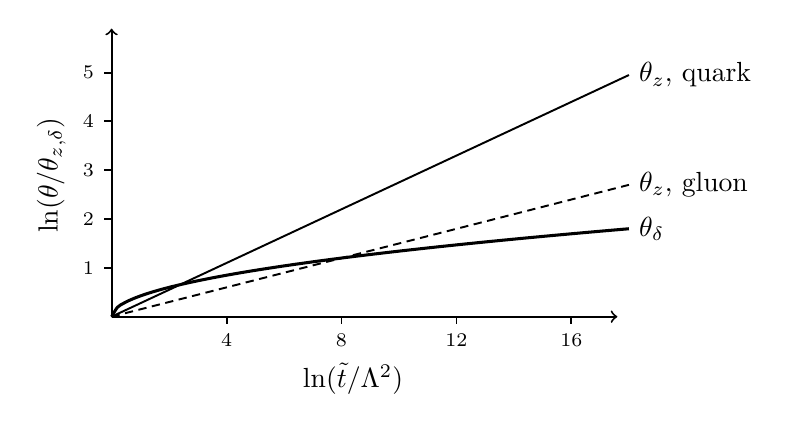
\begin{tikzpicture}[x=0.365cm, y=0.62cm, line width=0.7pt]
		\draw[->] (0,0) -- (17.6,0);
		\draw[->] (0,0) -- (0,5.9);
		\foreach \i in {4,8,12,16} {
			\draw (\i,0) -- (\i,-0.14) node[below] {\scriptsize\(\i\)};
		}
		\foreach \j in {1,2,3,4,5} {
			\draw (0,\j) -- (-0.26,\j) node[left] {\scriptsize\(\j\)};
		}
		\node[below] at (8.4,-0.75) {\(\ln(\tilde{t}/\Lambda^2)\)};
		\node[rotate=90] at (-2.1,2.9) {\(\ln(\theta/\theta_{z,\delta})\)};
		\draw[domain=0:18, samples=2] plot (\x, {0.275*\x});
		\draw[domain=0:18, samples=2, densely dashed] plot (\x, {0.150*\x});
		\draw[domain=0:18, samples=90, smooth, line width=1.1pt]
		plot (\x, {0.4245*sqrt(\x)});
		\node[right] at (18,4.95) {\(\theta_z\), quark};
		\node[right] at (18,2.70) {\(\theta_z\), gluon};
		\node[right] at (18,1.80) {\(\theta_\delta\)};
	\end{tikzpicture}
	\caption[Collimation of the energy and multiplicity flows of a jet]{%
		Collimation of the energy and of the multiplicity flow of a jet against its
		hardness, for \(z=0.9\), \(\delta=\tfrac12\), \(N_f=3\). The energy cone
		\(\theta_z\) of Eq.~\ref{eq:energyCollimation} closes linearly in
		\(\ln(\tilde{t}/\Lambda^2)\) and faster for quark jets; the multiplicity cone
		\(\theta_\delta\) of Eq.~\ref{eq:multCollimation} only as its square root.}
	\label{fig:collimationCones}
\end{figure}


The angularities of Chapter~\ref{ch:angularities} replace the cone by a weight, and
the same cascade fixes their distributions:
\begin{align}
	\lambda_\beta^\kappa &= \sum_{c\,\in J} z_c^\kappa
	\left(\frac{\Delta R_c}{R}\right)^{\beta} ,
	\qquad
	z_c = p_{\mathrm{T},c}\Big/\!\!\sum_{c^\prime\in J}p_{\mathrm{T},c^\prime} ,
	\notag\\
	dn &= \frac{2\alpha_s\mathbf{Q}_i^2}{\pi}\frac{dz}{z}\frac{d\theta}{\theta}
	= \frac{2\alpha_s\mathbf{Q}_i^2}{\pi}\,du\,dv ,
	\qquad
	u = \ln\frac{1}{z} , \qquad v = \ln\frac{R}{\theta} ,
	\label{eq:angularityDef}
\end{align}
the density being the single-emitter antenna pattern of
Eq.~\ref{eq:antennaSplitXSec} with \(\zeta\simeq\theta^2/2\), uniform on the quadrant,
each emission contributing \(z^\kappa(\theta/R)^\beta\) to the sum, which at this
accuracy is dominated by one of them. Let \(\Sigma_i(\lambda)\) be the fraction of
jets whose angularity falls below a value \(\lambda\). At \(\kappa=1\) an emission
carries \(\lambda^1_\beta\) above \(\lambda\) when \(u+\beta v<\ln(1/\lambda)\), a
triangle of area \(\ln^2(1/\lambda)/2\beta\), and vetoing every such emission gives
\begin{equation}
	\Sigma_i(\lambda) = \exp\left[-\frac{\alpha_s\mathbf{Q}_i^2}{\pi\beta}
	\ln^2\frac{1}{\lambda}\right] ,
	\qquad
	\Sigma_g(\lambda) = \left[\Sigma_q(\lambda)\right]^{C_A/C_F} ,
	\label{eq:angularitySudakov}
\end{equation}
a Sudakov form factor vetoing an observable rather than a cone, and at \(\beta=1\) the
double-logarithmic thrust distribution~\cite{Ellis_Stirling_Webber_1996e}. Equations~\ref{eq:swWidth} and
\ref{eq:angularitySudakov} invert one another. At \(\kappa=0\) the vetoed region is
instead the strip \(v<\ln(1/\lambda)/\beta\), unbounded in \(u\): nothing
exponentiates and \(\lambda^0_\beta\) counts emissions, governed by
Eq.~\ref{eq:dlaMultiplicity}. So \(\lambda^1_1\) is the jet width and measures
\(\theta_z\), \(\lambda^0_0\) the jet multiplicity and \(\theta_\delta\), and
\((\kappa,\beta)\) carries one into the other --- with the quark--gluon memory at
large \(u\), small \(v\), exactly where grooming cuts, so the quark and gluon
fractions of a sample must be fixed before a change in its angular structure is read
as a medium effect.








%===========================================================================================


